\documentclass{beamer}
\usepackage[latin1]{inputenc}
\usepackage{alltt}
\usepackage{color}
\definecolor{type}{rgb}{0.25,0.5,0.25}
\usetheme{Frankfurt} %{Warsaw}
\title[Lisaac]{Lisaac}
\subtitle{{\it{}Efficient compilation strategy for object-oriented languages\\
under the closed-world assumption}}
\author{Beno�t Sonntag -- benoit.sonntag@lisaac.org}
\institute{

\includegraphics[scale=0.6]{figures/isaac_logo.eps} \\
\url{http://www.lisaac.org} \\
}
\date{\vspace{-5ex}}

\begin{document}
%---------------------------------------------------
\begin{frame}
\titlepage
\end{frame}
%---------------------------------------------------
\AtBeginSubsection[]
{
  \begin{frame}<beamer>
    \frametitle{Plan}
    \tableofcontents[currentsection,currentsubsection]
  \end{frame}
}
%---------------------------------------------------
\section{Introduction}
%===============================
%---------------------------------------------------
\begin{frame}{History\,: Lisaac for IsaacOOS Language}
\begin{columns}
\begin{column}[l]{5cm}
\begin{block}{In the past\ldots}
\begin{center}
{\bf{}C} language\\
$\Downarrow$\\
{\bf{}Unix} system
\end{center}
\end{block}
\end{column}
\begin{column}[r]{5cm}
\begin{block}{The futur\ldots}
\begin{center}
{\bf{}Lisaac}\\
{\it{}Prototype based Object Oriented Language}\\
$\Downarrow$\\
{\bf{}IsaacOOS}\\
{\it{}Prototype Object Operating System}
\end{center}
\end{block}
\end{column}
\end{columns}
\end{frame}
%---------------------------------------------------
\begin{frame}{Let them sink in a bigger box ?}
\begin{center}
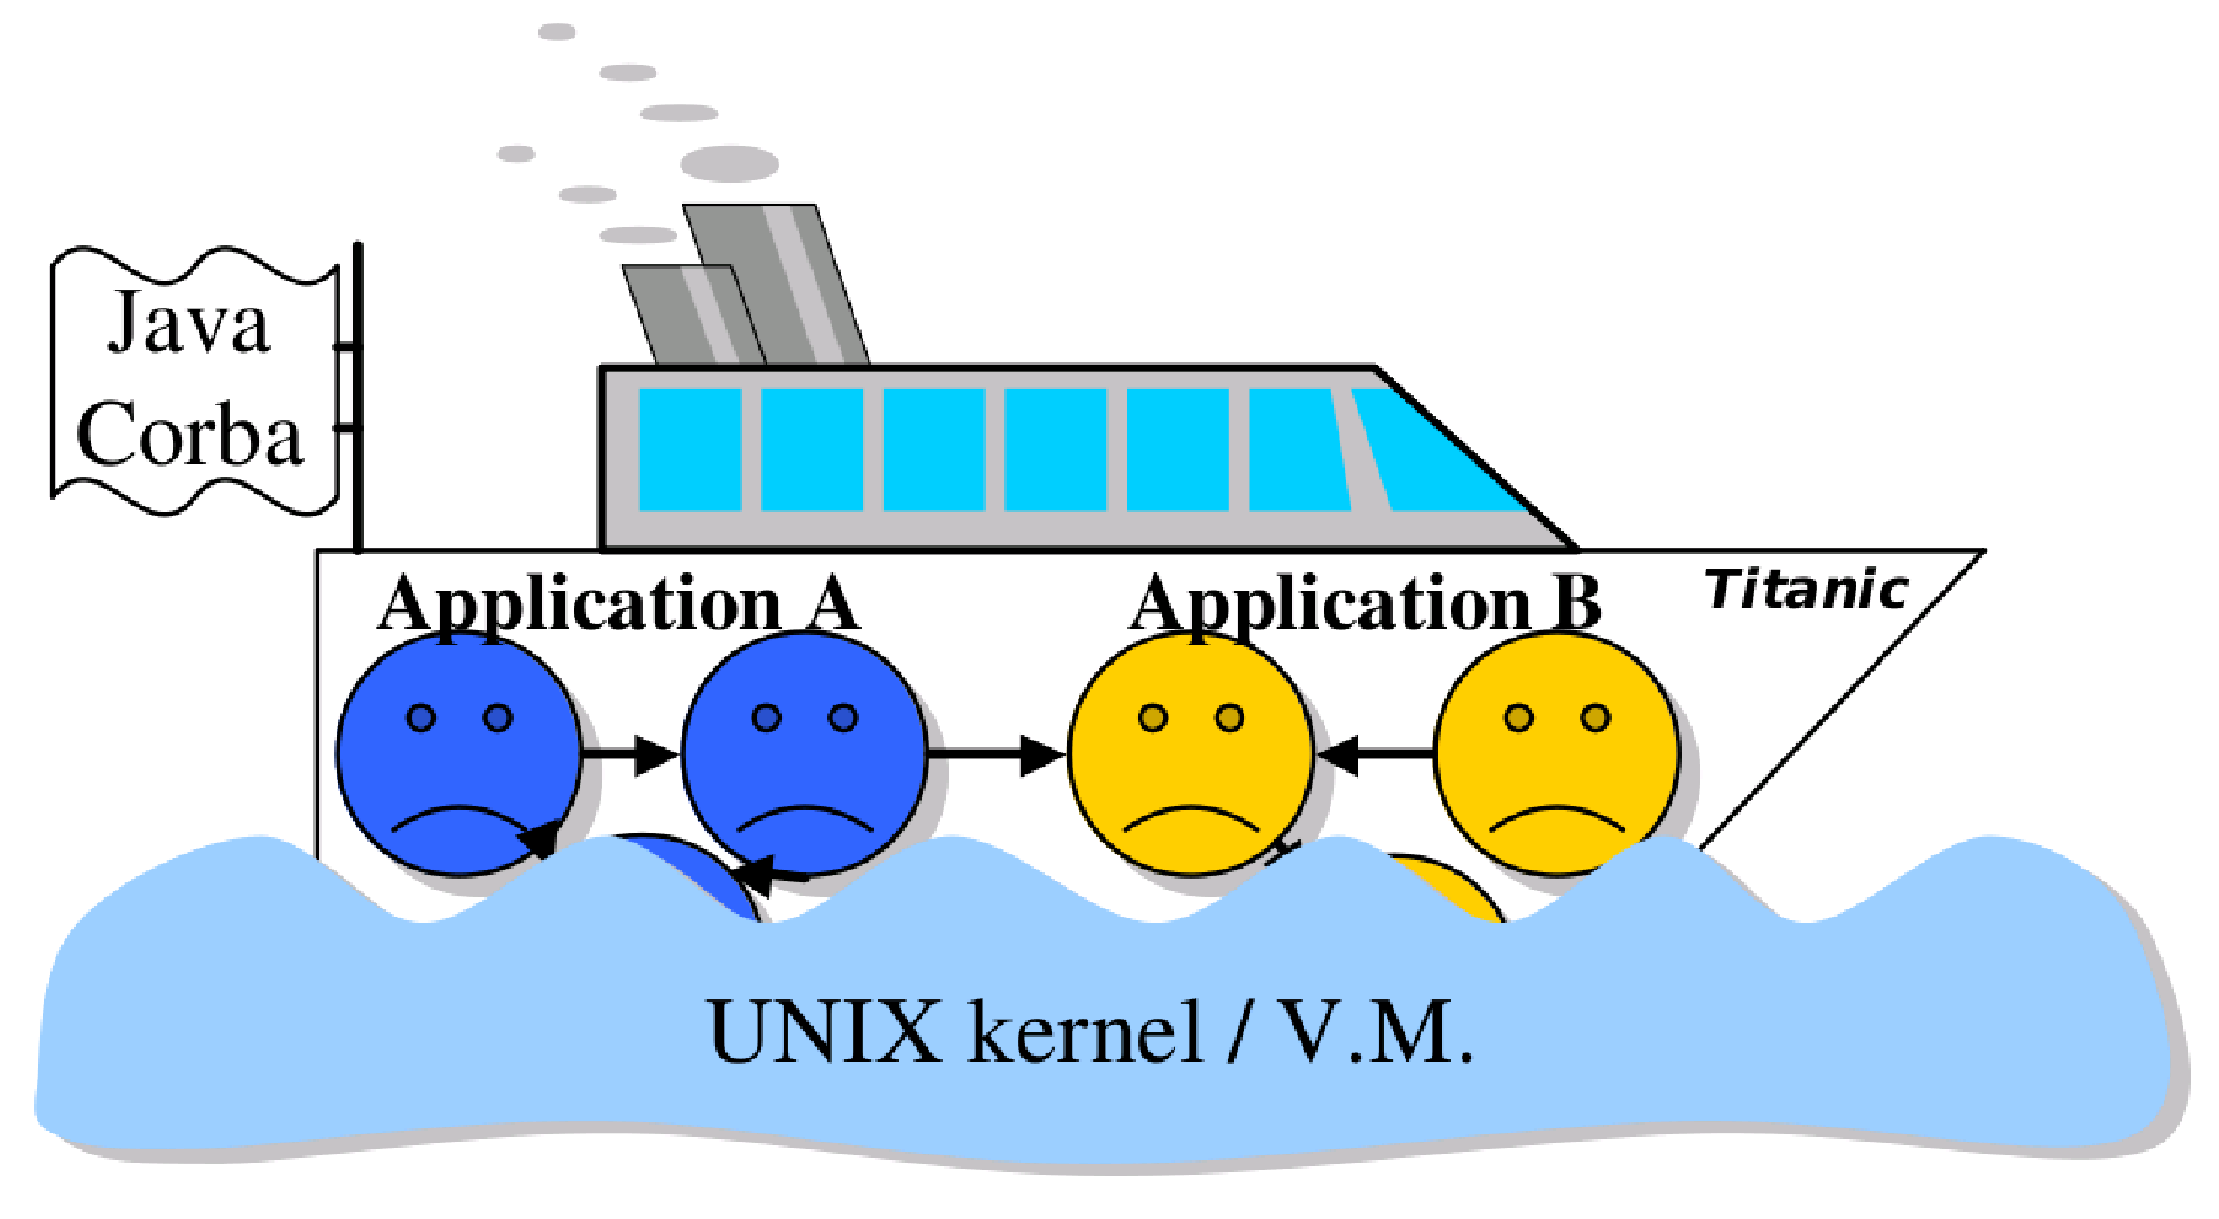
\includegraphics[scale=0.3]{figures/boat.eps}
\end{center}
\end{frame}
%---------------------------------------------------
\begin{frame}{High-level {\it{}vs} Hardware}
{\bf{}Object Oriented for Hardware}
\begin{center}
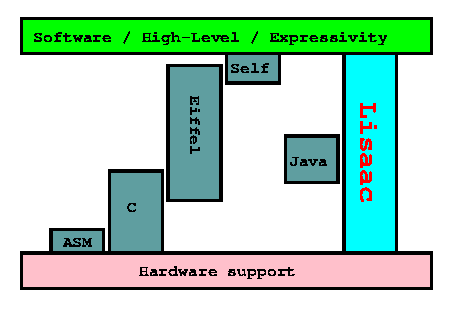
\includegraphics[scale=1.2]{figures/high_level.eps}
\end{center}
\end{frame}
%---------------------------------------------------
\begin{frame}{Class {\it{}vs} Prototype (1/3)}
\begin{block}{Class}
\begin{center}
\includegraphics[scale=1.0]{figures/class_proto.eps}
\end{center}
\end{block}
\begin{block}{Prototype}
\begin{center}
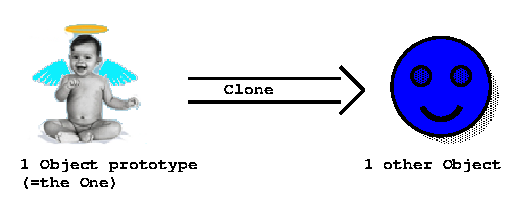
\includegraphics[scale=1.0]{figures/proto.eps}
\end{center}
\end{block}
\end{frame}
%---------------------------------------------------
\begin{frame}{Class {\it{}vs} Prototype (2/3)}
\begin{columns}
\begin{column}[l]{5.5cm}
\begin{block}{Class}
 \includegraphics[scale=0.9]{figures/herit_class.eps}
\end{block}
\end{column}
\begin{column}[r]{5.5cm}
\begin{block}{Prototype}
 \includegraphics[scale=0.9]{figures/herit_proto.eps}
\end{block}
\end{column}
\end{columns}
\end{frame}
%---------------------------------------------------
\begin{frame}{Class {\it{}vs} Prototype (3/3)}
\begin{block}{Dynamic inheritance}
\begin{center}
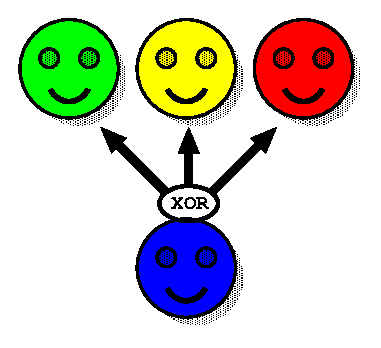
\includegraphics[scale=1.0]{figures/inherit.eps}
\end{center}
\end{block}
\end{frame}
%---------------------------------------------------

\section{The language}
%=====================
%---------------------------------------------------
%\begin{frame}{The grammar of Lisaac}
%\begin{center}
%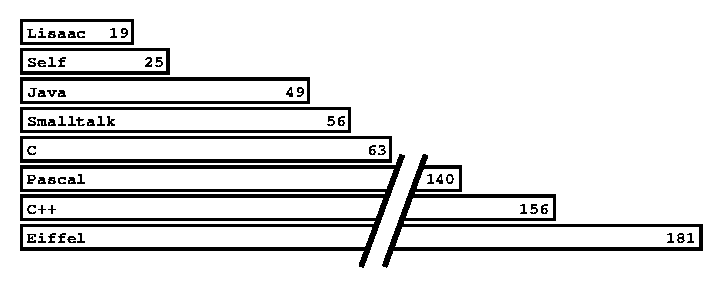
\includegraphics[scale=1.0]{figures/grammar.eps}\\
%{\it{}Number of gamatical rules}
%\end{center}
%\end{frame}
%---------------------------------------------------
\begin{frame}{Example\,: Hello world!}
\begin{block}{\tt{}hello.li}
\begin{alltt}
\textcolor{red}{Section Header}\\
~~\textcolor{red}{$+$} \textcolor{blue}{name} := \textcolor{type}{HELLO};\\
\textcolor{red}{Section Public}\\
~~\textcolor{red}{$-$} \textcolor{blue}{main} $<-$ \\
~~(\\
~~~~(1+2).print;\\
~~~~'A'.print;\\
~~~~``Hello world !$\backslash$n''.\textcolor{blue}{print};\\
~~);\\
\end{alltt}
\end{block}
{\it{}Command line\,:} {\tt{}lisaac hello.li}\\
{\it{}Executable result\,:} {\tt{}hello} {\it{}(ou {\tt{}hello.exe} for windows)}\\
\end{frame}
%---------------------------------------------------
\begin{frame}{Slot identifier}
\begin{alltt}
\textcolor{red}{$-$}\,\textcolor{blue}{qsort}\,tab:\textcolor{type}{COLLECTION}\,\textcolor{blue}{from}\,low:\textcolor{type}{INTEGER}\,\textcolor{blue}{to}\,high:\textcolor{type}{INTEGER}\,$\leftarrow$ \\
( \textcolor{red}{+} i,j:\textcolor{type}{INTEGER};\\
~~\textcolor{red}{+} x,y:\textcolor{type}{OBJECT};\\
~~i := low;\\
~~j := high;\\
~~x := tab.\textcolor{blue}{item} ((i + j)$>>$ 1);\\
~~\{ \ldots\\
~~~~(i $<=$ j).\textcolor{blue}{if} \{\\
~~~~~~tab.\textcolor{blue}{swap} j \textcolor{blue}{and} i;\\
~~~~~~\ldots\\
~~~~\};\\
~~\}.\textcolor{blue}{do\_while} \{i $<=$ j\};\\
~~(low $<$ j).\textcolor{blue}{if} \{ \textcolor{blue}{qsort} tab \textcolor{blue}{from} low \textcolor{blue}{to} j; \};\\
~~(i $<$ high).\textcolor{blue}{if} \{ \textcolor{blue}{qsort} tab \textcolor{blue}{from} i \textcolor{blue}{to} high; \};\\
);\\
\end{alltt}
\end{frame}
%---------------------------------------------------
\begin{frame}{Slot identifier}
\begin{alltt}
\textcolor{red}{$-$}\,\colorbox{red}{\textcolor{blue}{qsort}}\,tab:\textcolor{type}{COLLECTION}\,\colorbox{red}{\textcolor{blue}{from}}\,low:\textcolor{type}{INTEGER}\,\colorbox{red}{\textcolor{blue}{to}}\,high:\textcolor{type}{INTEGER}\,$\leftarrow$ \\
( \textcolor{red}{+} i,j:\textcolor{type}{INTEGER};\\
~~\textcolor{red}{+} x,y:\textcolor{type}{OBJECT};\\
~~i := low;\\
~~j := high;\\
~~x := tab.\textcolor{blue}{item} ((i + j)$>>$ 1);\\
~~\{ \ldots\\
~~~~(i $<=$ j).\textcolor{blue}{if} \{\\
~~~~~~tab.\textcolor{blue}{swap} j \textcolor{blue}{and} i;\\
~~~~~~\ldots\\
~~~~\};\\
~~\}.\textcolor{blue}{do\_while} \{i $<=$ j\};\\
~~(low $<$ j).\textcolor{blue}{if} \{ \colorbox{red}{\textcolor{blue}{qsort}} tab \colorbox{red}{\textcolor{blue}{from}} low \colorbox{red}{\textcolor{blue}{to}} j; \};\\
~~(i $<$ high).\textcolor{blue}{if} \{ \colorbox{red}{\textcolor{blue}{qsort}} tab \colorbox{red}{\textcolor{blue}{from}} i \colorbox{red}{\textcolor{blue}{to}} high; \};\\
);\\
\end{alltt}
\end{frame}
%---------------------------------------------------
\begin{frame}{Slot identifier\,: if}
\begin{alltt}
\textcolor{red}{$-$}\,\textcolor{blue}{qsort}\,tab:\textcolor{type}{COLLECTION}\,\textcolor{blue}{from}\,low:\textcolor{type}{INTEGER}\,\textcolor{blue}{to}\,high:\textcolor{type}{INTEGER}\,$\leftarrow$ \\
( \textcolor{red}{+} i,j:\textcolor{type}{INTEGER};\\
~~\textcolor{red}{+} x,y:\textcolor{type}{OBJECT};\\
~~i := low;\\
~~j := high;\\
~~x := tab.\textcolor{blue}{item} ((i + j)$>>$ 1);\\
~~\{ \ldots\\
~~~~(i $<=$ j).\colorbox{red}{\textcolor{blue}{if} \{}\\
~~~~~~tab.textcolor{blue}{swap} j \textcolor{blue}{and} i;\\
~~~~~~\ldots\\
~~~~\colorbox{red}{\}};\\
~~\}.\textcolor{blue}{do\_while} \{i $<=$ j\};\\
~~(low $<$ j).\textcolor{blue}{if} \{ \textcolor{blue}{qsort} tab \textcolor{blue}{from} low \textcolor{blue}{to} j; \};\\
~~(i $<$ high).\textcolor{blue}{if} \{ \textcolor{blue}{qsort} tab \textcolor{blue}{from} i \textcolor{blue}{to} high; \};\\
);\\
\end{alltt}
\end{frame}
%---------------------------------------------------
\begin{frame}{Slot identifier\,: loop}
\begin{alltt}
\textcolor{red}{$-$}\,\textcolor{blue}{qsort}\,tab:\textcolor{type}{COLLECTION}\,\textcolor{blue}{from}\,low:\textcolor{type}{INTEGER}\,\textcolor{blue}{to}\,high:\textcolor{type}{INTEGER}\,$\leftarrow$ \\
( \textcolor{red}{+} i,j:\textcolor{type}{INTEGER};\\
~~\textcolor{red}{+} x,y:\textcolor{type}{OBJECT};\\
~~i := low;\\
~~j := high;\\
~~x := tab.\textcolor{blue}{item} ((i + j)$>>$ 1);\\
~~\colorbox{red}{\{} \ldots\\
~~~~(i $<=$ j).\textcolor{blue}{if} \{\\
~~~~~~tab.\textcolor{blue}{swap} j \textcolor{blue}{and} i;\\
~~~~~~\ldots\\
~~~~\};\\
~~\colorbox{red}{\}.\textcolor{blue}{do\_while} \{i $<=$ j\};}\\
~~(low $<$ j).\textcolor{blue}{if} \{ \textcolor{blue}{qsort} tab \textcolor{blue}{from} low \textcolor{blue}{to} j; \};\\
~~(i $<$ high).\textcolor{blue}{if} \{ \textcolor{blue}{qsort} tab \textcolor{blue}{from} i \textcolor{blue}{to} high; \};\\
);\\
\end{alltt}
\end{frame}
%---------------------------------------------------
\begin{frame}{If then else}
%\hspace{-5cm}
\includegraphics[scale=0.48]{figures/if_then_else.ps}
\end{frame}
%---------------------------------------------------
\begin{frame}{Assignment\,: code}
\begin{block}{Example}
\begin{columns}
\begin{column}[l]{6cm}
\begin{alltt}
\textcolor{red}{$-$} \textcolor{blue}{color} (r,g,b:\textcolor{type}{INTEGER}) $<-$ \\
( \\
~~\textcolor{blue}{true\_color}:=r$<<$16|g$<<$8|b;\\
);\\
\ldots\\
( \\
~~\textcolor{blue}{color} $<-$ (\\
~~~~\textcolor{blue}{gray\_color} := (r+g+b)/3;\\
~~);\\
);\\
\end{alltt}
\end{column}
\begin{column}[r]{4cm}
\includegraphics[scale=0.175]{figures/flower.ps}
\end{column}
\end{columns}
\end{block}
\end{frame}
%---------------------------------------------------
\begin{frame}{Inheritance\,: Dynamic once compute parent}
\begin{block}{Once execution dynamic parent evaluation}
\begin{alltt}
\textcolor{red}{Section Inherit}\\
~~\textcolor{red}{$+$} \textcolor{blue}{parent}:\textcolor{type}{OBJECT} $<-$\\
~~( \textcolor{red}{$+$} result:\textcolor{type}{OBJECT};\\
~~~~\ldots  // {\it{} compute my parent}\\
~~~~\textcolor{blue}{parent} := result  // {\it{}my parent is a data now!!!}\\
~~);\\
\end{alltt}
\end{block}
\begin{exampleblock}{Note}
\begin{itemize}
\item The first lookup, the parent is dynamically defined
\item The next lookup, the parent is a simple data value
\end{itemize}
\end{exampleblock}
\end{frame}
%---------------------------------------------------

\section{Compiler}
%===============================
%---------------------------------------------------
\begin{frame}{Multi-platform compiler}
\includegraphics[scale=0.5]{figures/multiplatform.ps}
\end{frame}
%---------------------------------------------------
\begin{frame}{Global analysis}
\begin{block}{Java, C$++$\,: Classic technical}
Virtual Function Table (VFT)\\
$\Rightarrow$ Pointer of function\\
$\Rightarrow$ Indirect call\\
$\Rightarrow$ {\bf{}No optimization!}\\
\end{block}

\begin{alertblock}{Lisaac\,: Global analysis}
Transitive closure\\
$\Rightarrow$ Dispatch Binary Branch (DBB)\\
$\Rightarrow$ Static call\\
$\Rightarrow$ {\bf{}Full optimization!}\\
\end{alertblock}
\end{frame}
%---------------------------------------------------
\begin{frame}{Global overview}
\begin{center}
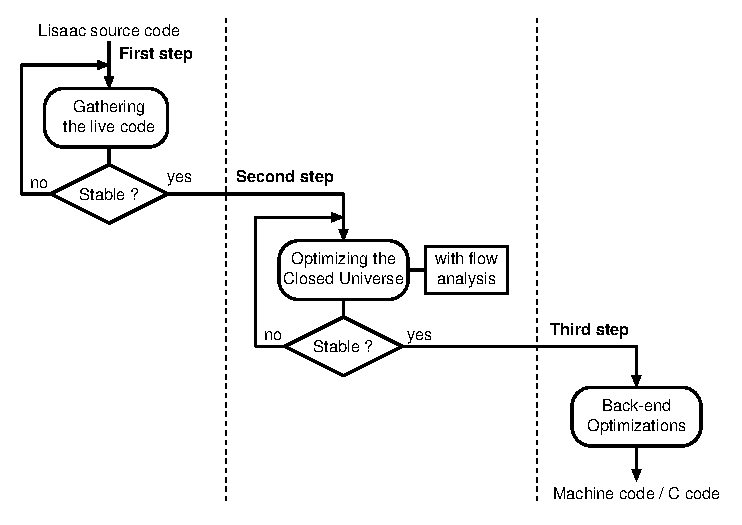
\includegraphics[scale=0.8]{figures/overview.eps}
\end{center}
\end{frame}
%---------------------------------------------------
\begin{frame}{Dispatch Binary Branch (1/4)}
\includegraphics[scale=0.5]{figures/dbb1.ps}
\end{frame}
%---------------------------------------------------
\begin{frame}{Dispatch Binary Branch (2/4)}
\includegraphics[scale=0.5]{figures/dbb2.ps}
\end{frame}
%---------------------------------------------------
\begin{frame}{Dispatch Binary Branch (3/4)}
\includegraphics[scale=0.5]{figures/dbb3.ps}
\end{frame}
%---------------------------------------------------
\begin{frame}{DBB: If then else}
\begin{center}
\includegraphics[scale=0.25]{figures/if_then_else_compiler.ps}
\end{center}
\end{frame}
%---------------------------------------------------
\begin{frame}{Dispatch Binary Branch (4/4)}
\includegraphics[scale=0.3]{figures/dbb_bench.ps}
\end{frame}
%---------------------------------------------------
\begin{frame}{Customization (1/6)}
\includegraphics[scale=0.25]{figures/cutomization_1.eps}
\end{frame}
%---------------------------------------------------
\begin{frame}{Customization: Call \#1 (2/6)}
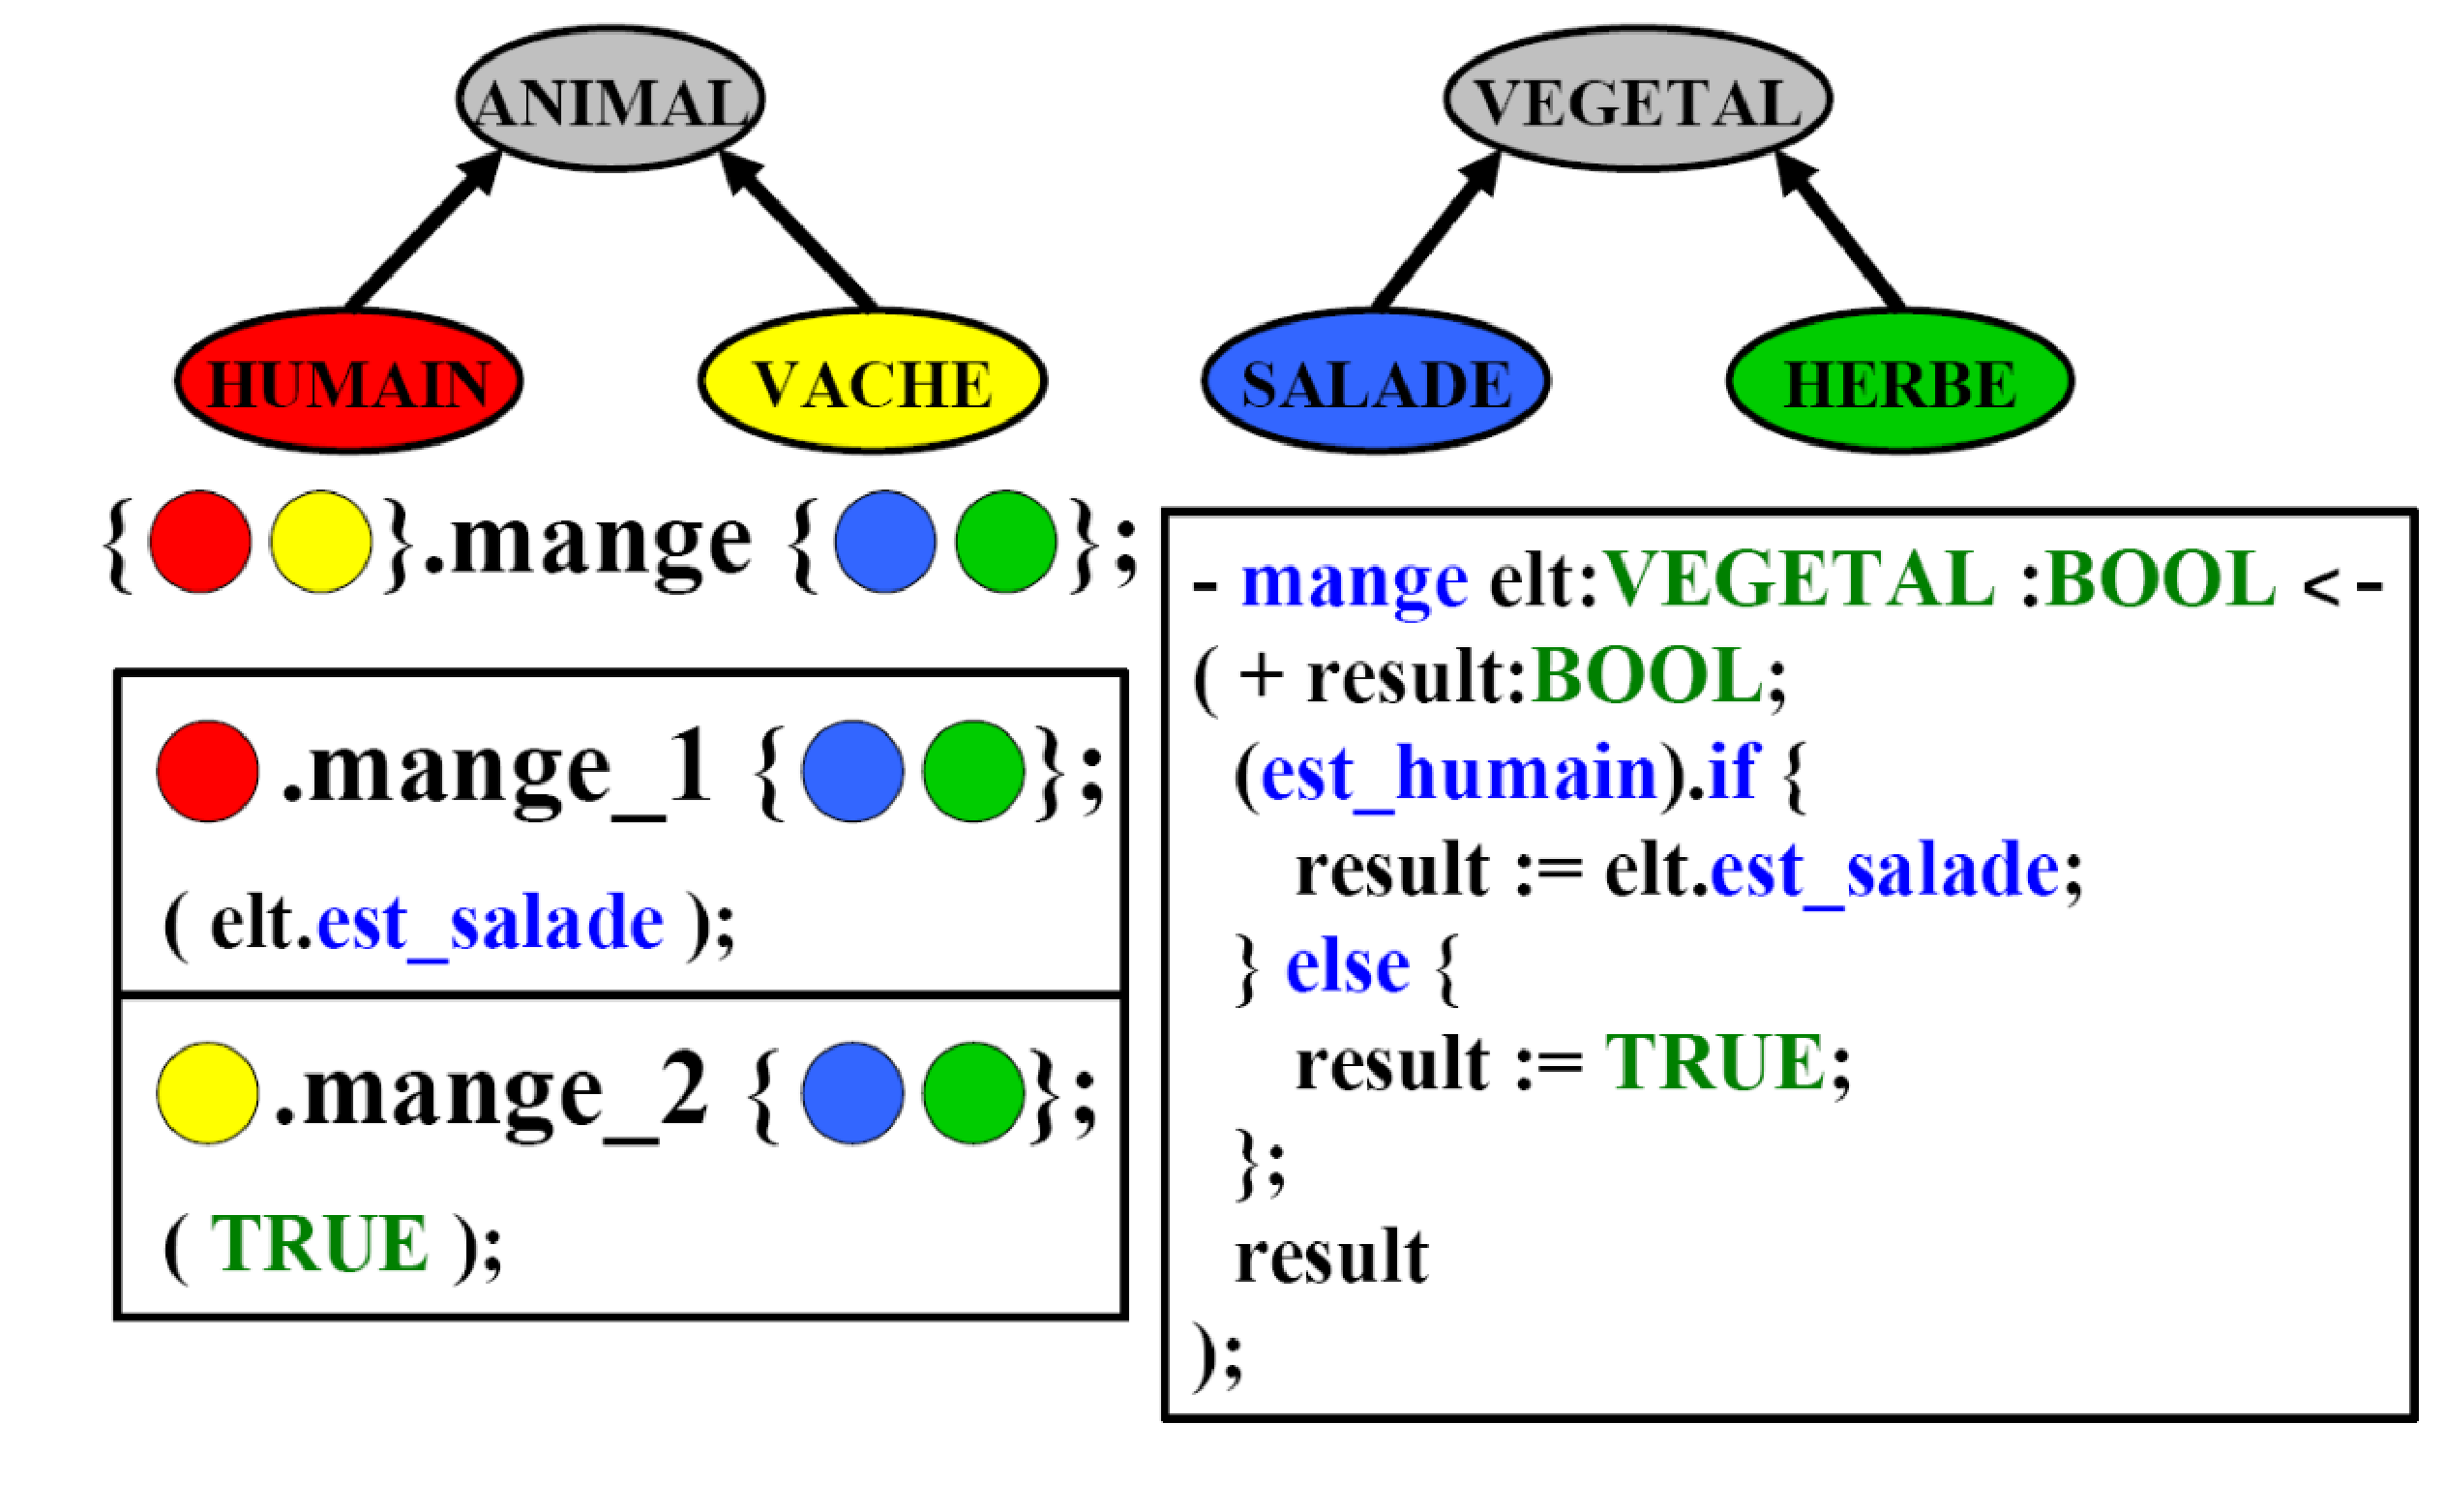
\includegraphics[scale=0.25]{figures/cutomization_2.eps}
\end{frame}
%---------------------------------------------------
\begin{frame}{Customization: Call \#2 (3/6)}
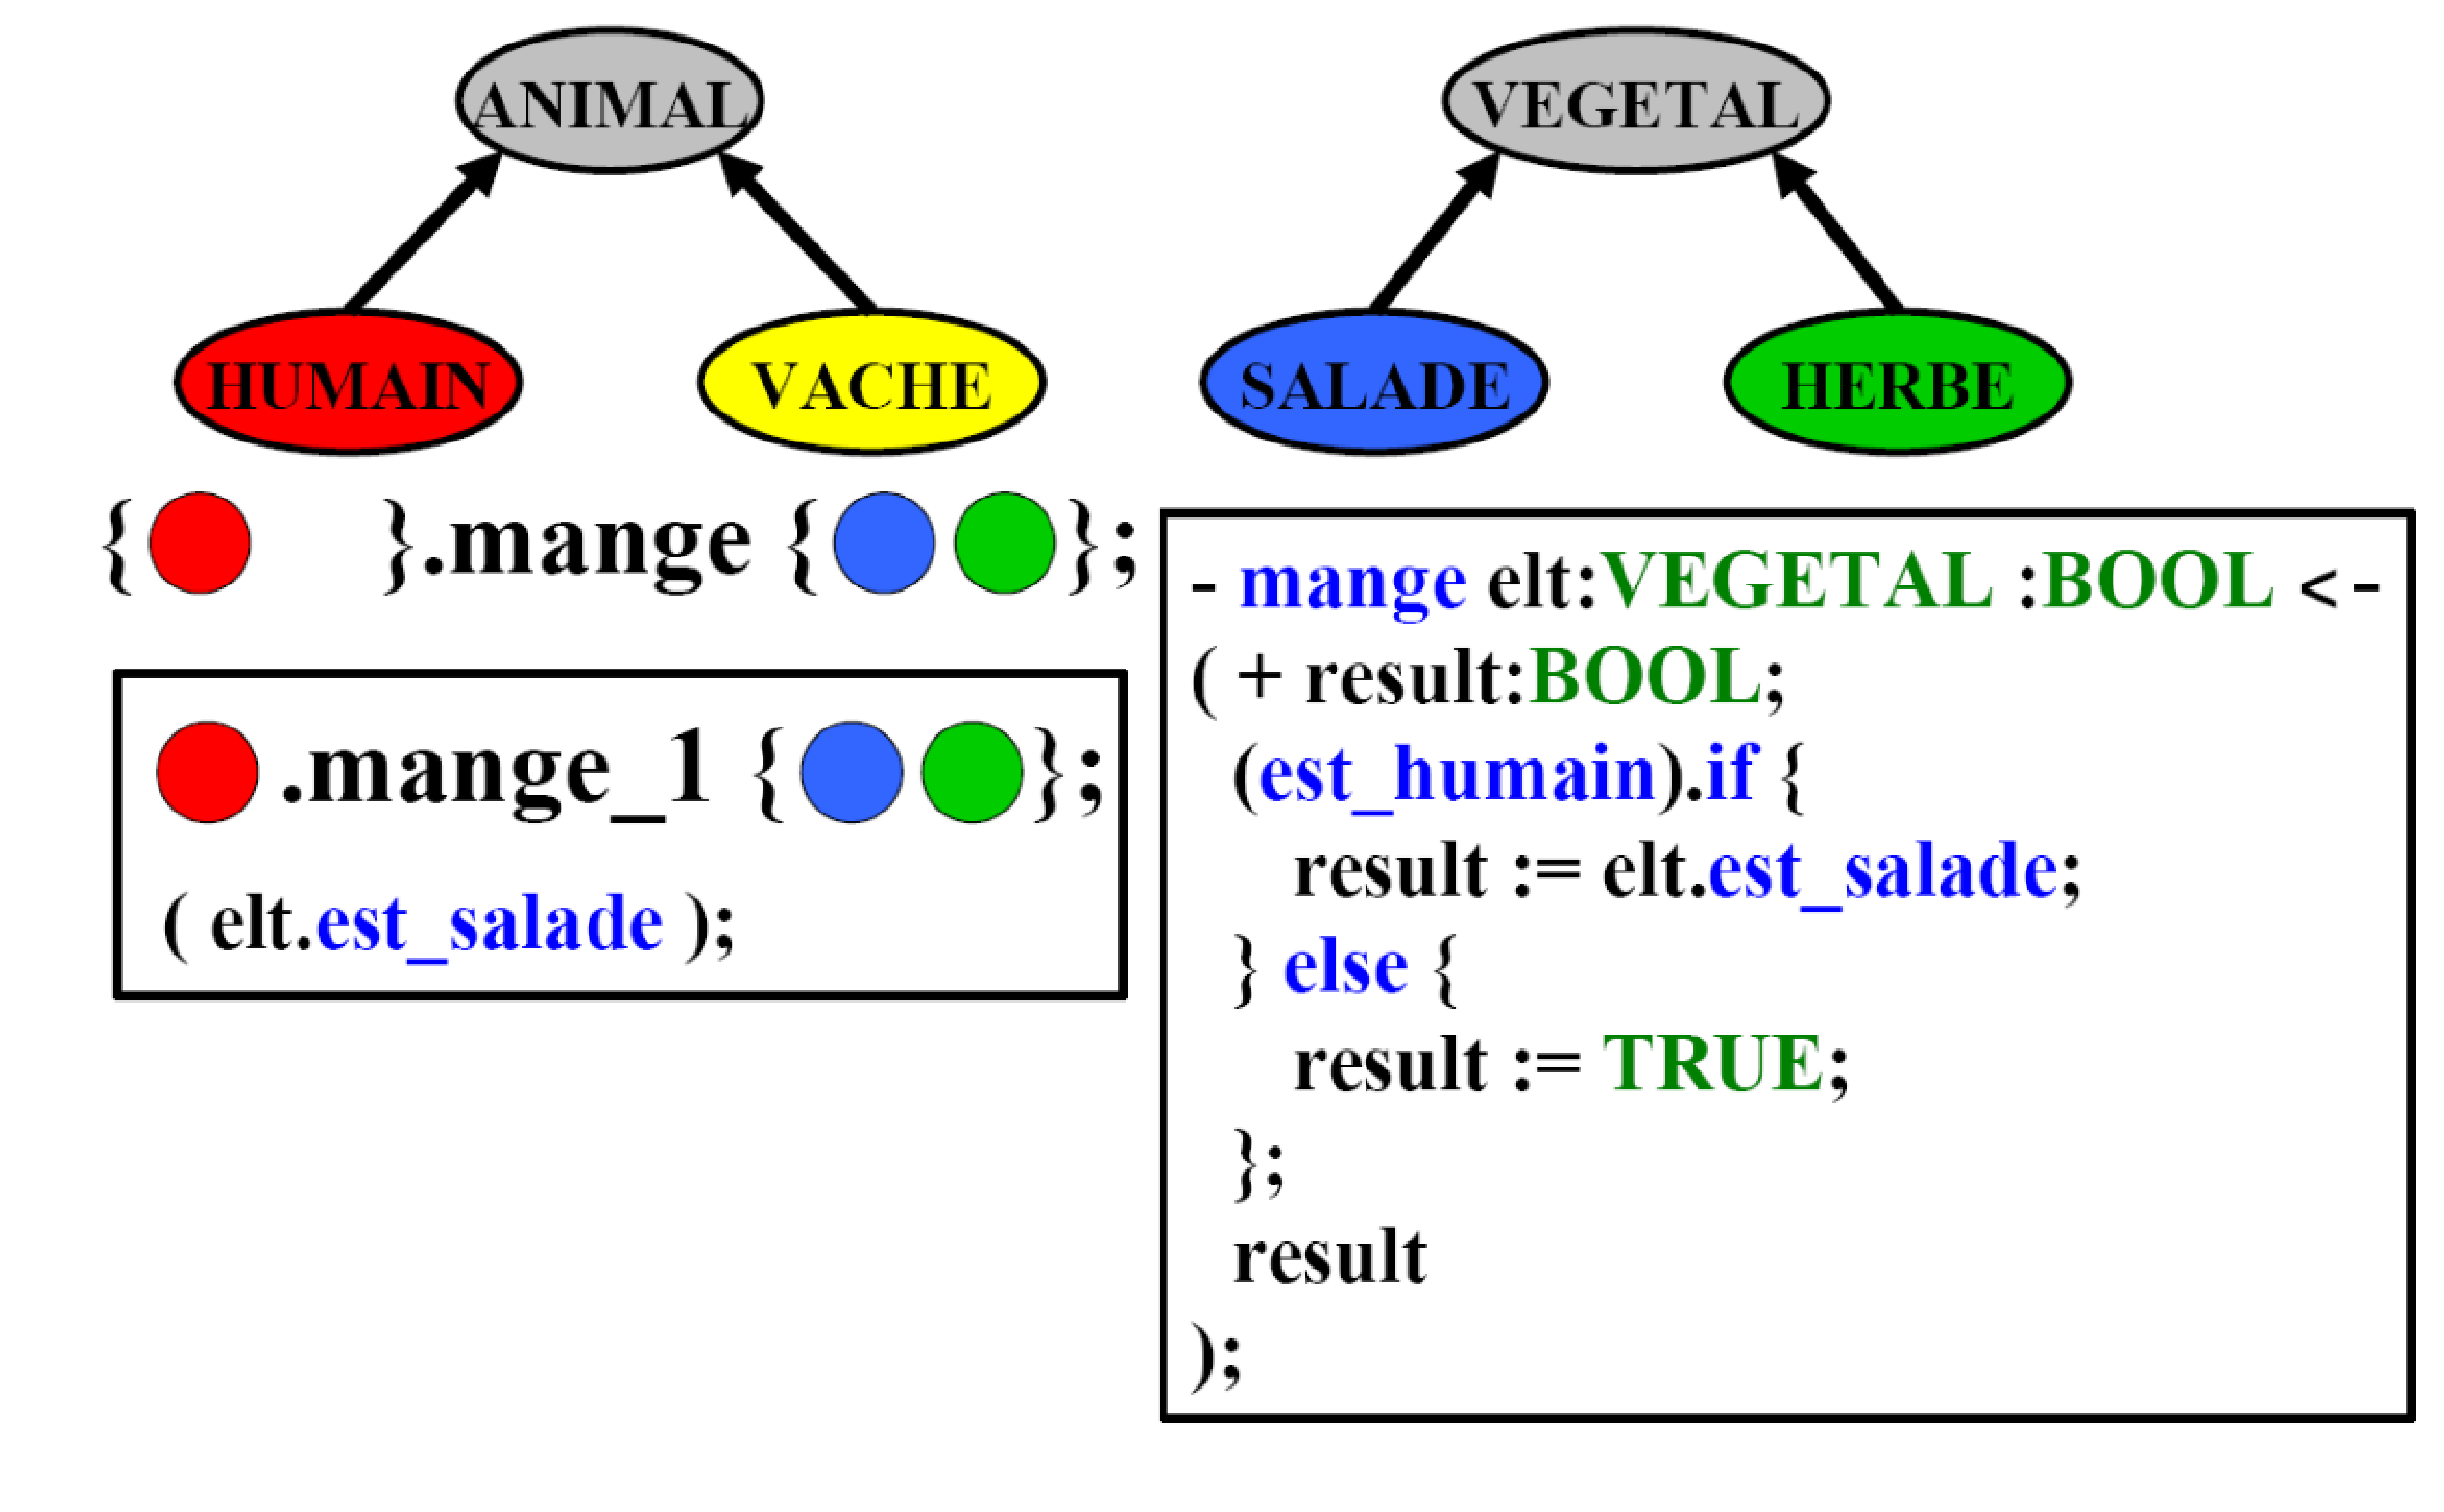
\includegraphics[scale=0.25]{figures/cutomization_3.eps}
\end{frame}
%---------------------------------------------------
\begin{frame}{Customization: Call \#3 (4/6)}
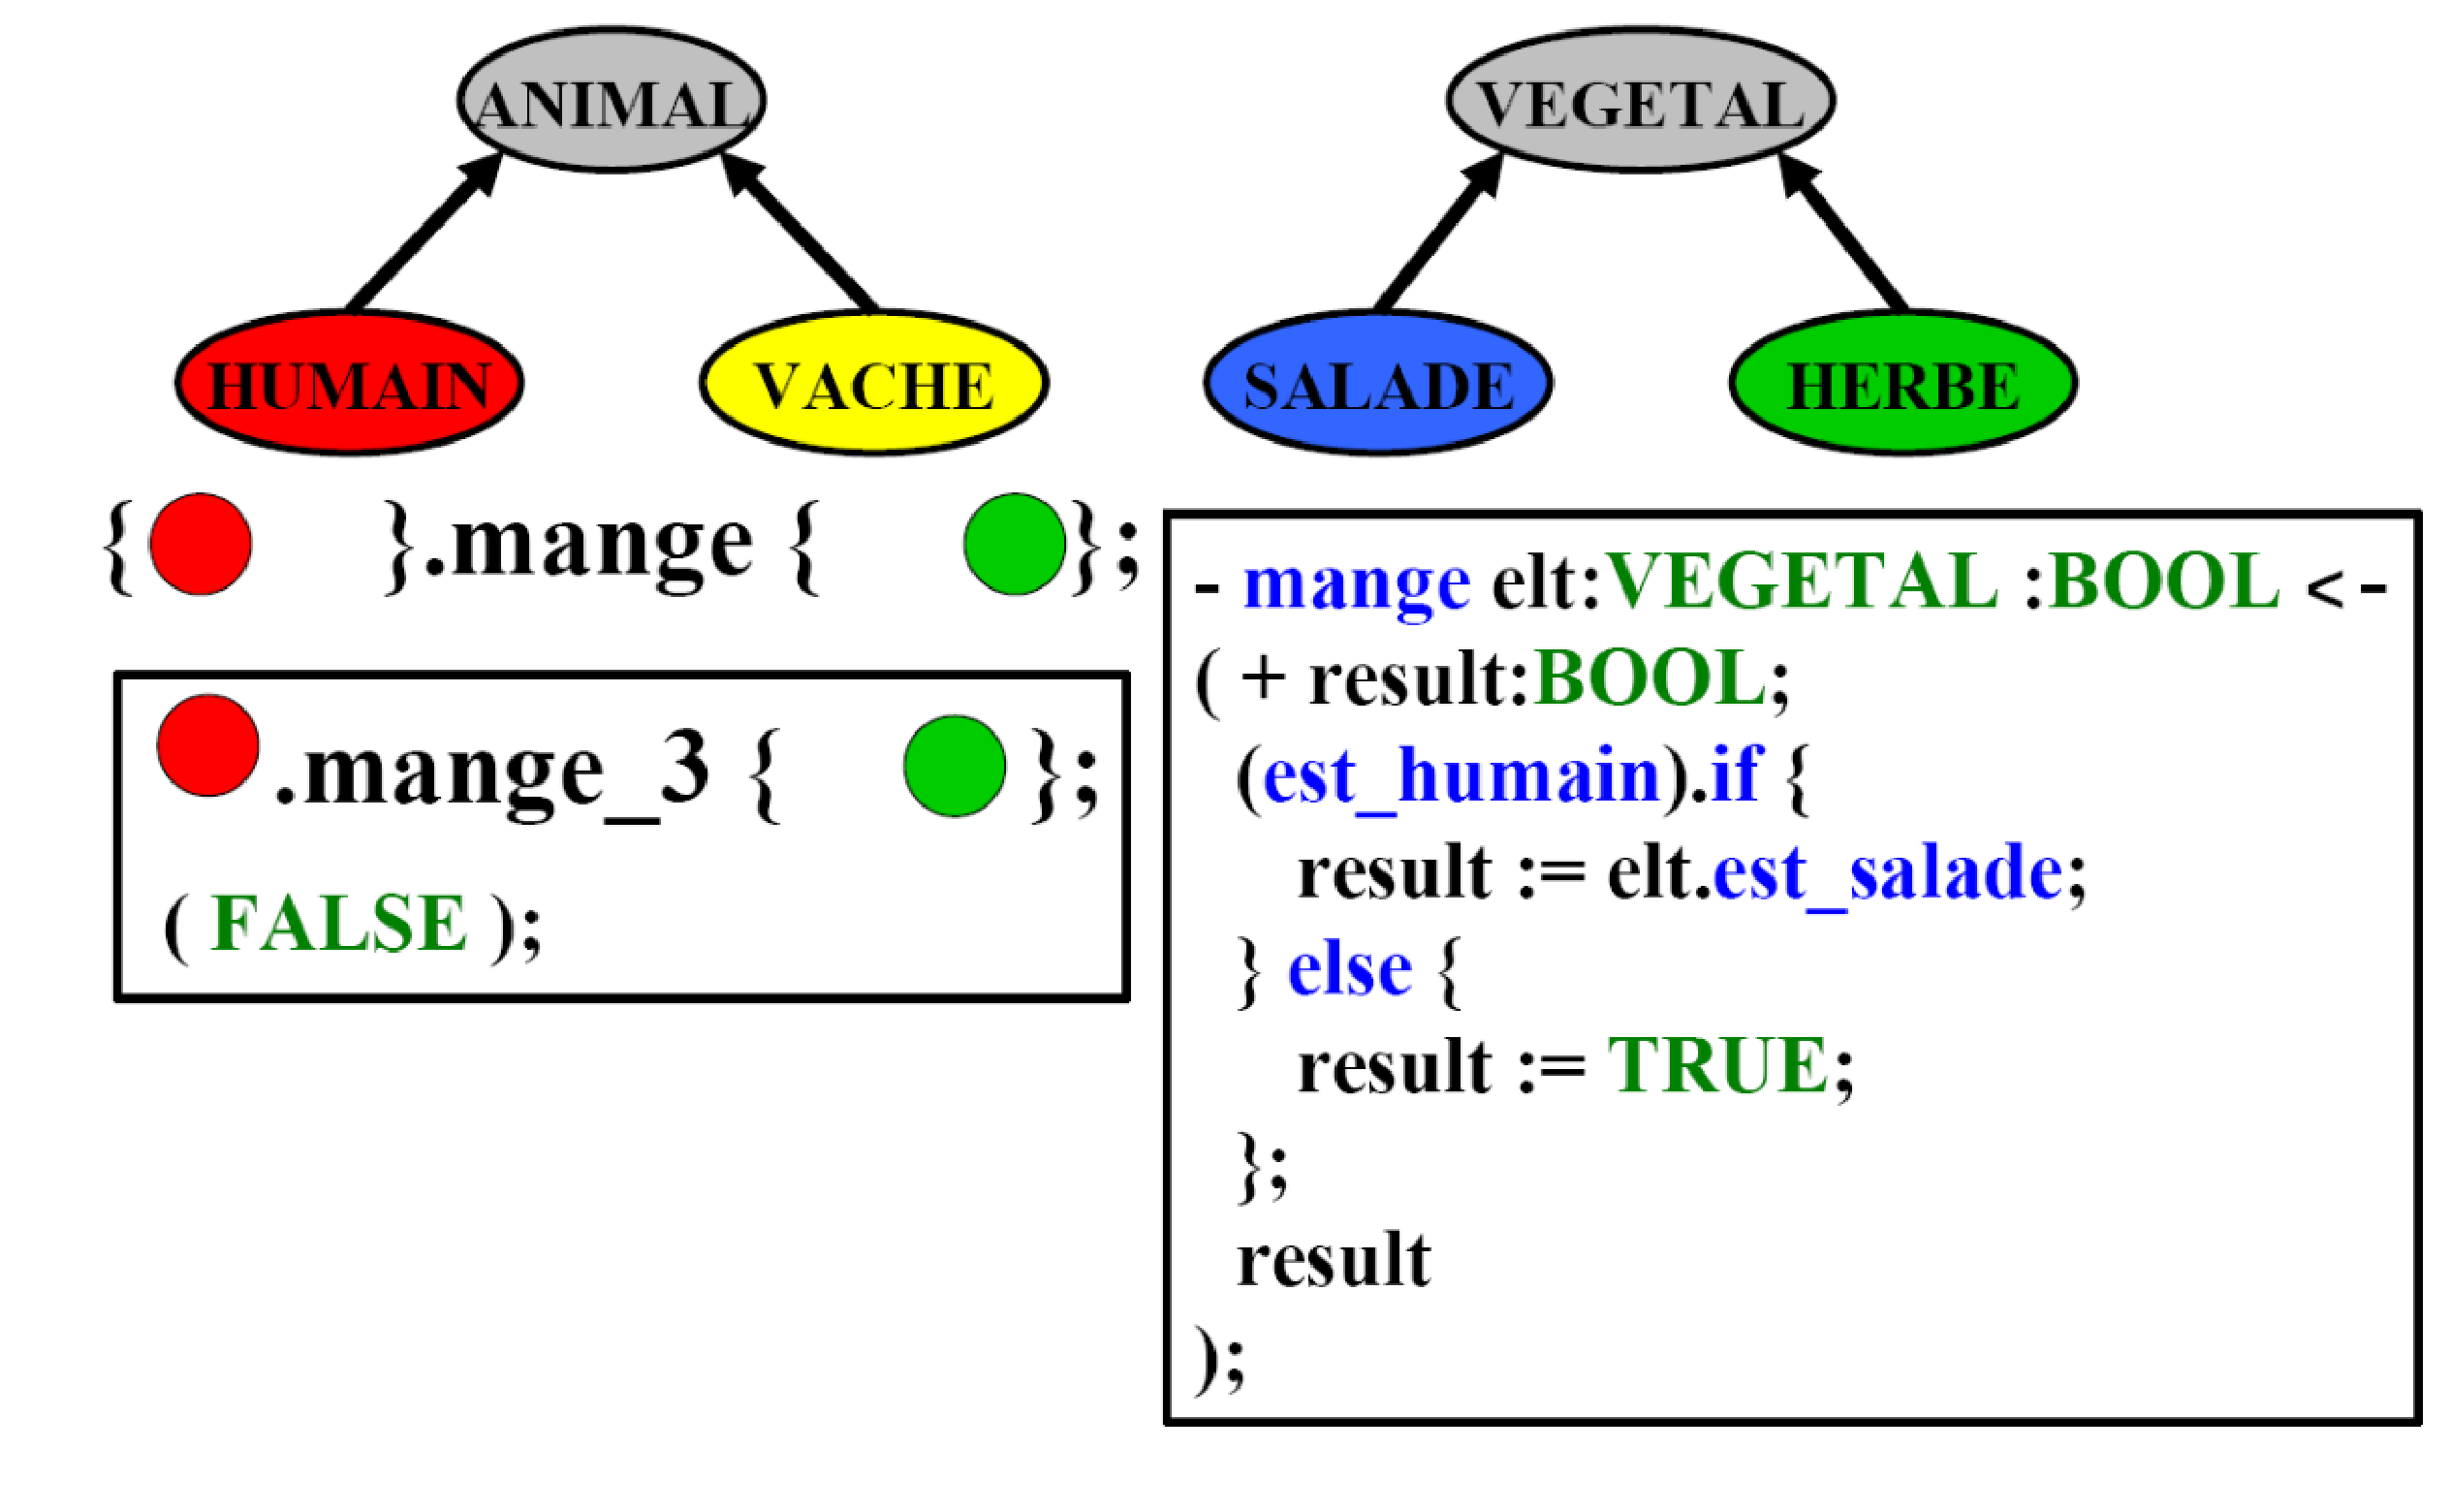
\includegraphics[scale=0.25]{figures/cutomization_4.eps}
\end{frame}
%---------------------------------------------------
\begin{frame}{Customization (5/6)}
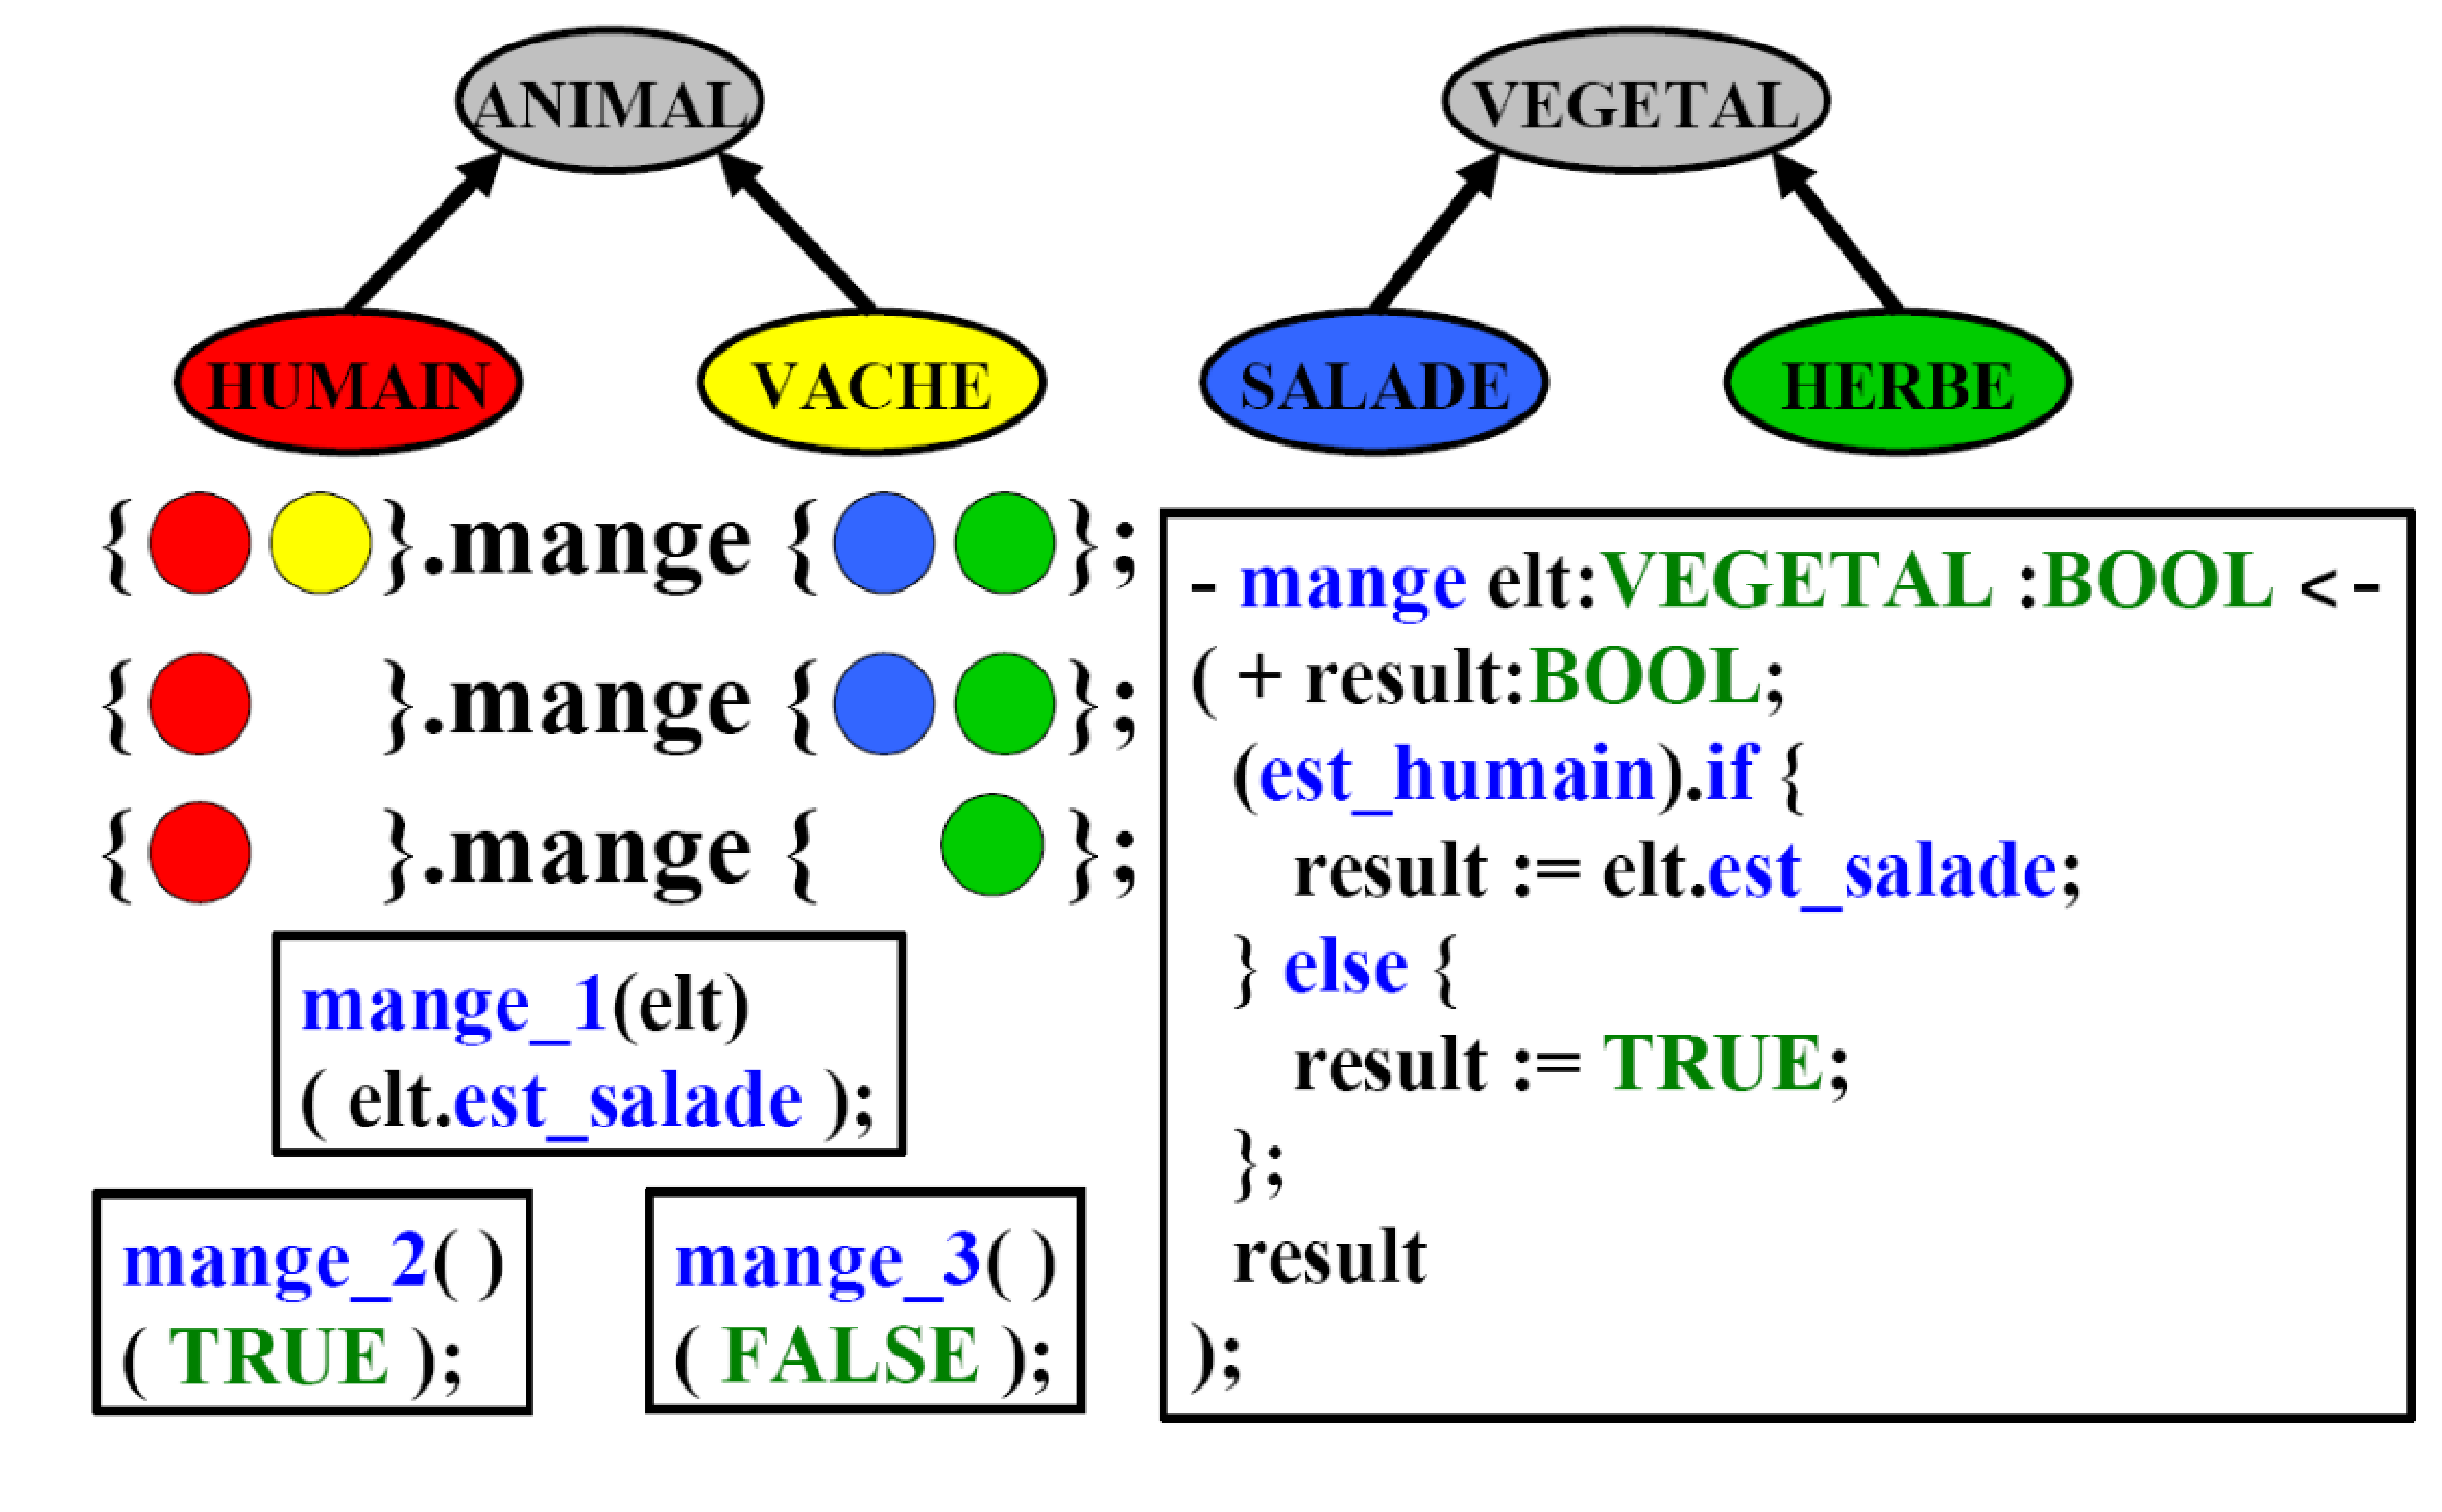
\includegraphics[scale=0.25]{figures/cutomization_5.eps}
\end{frame}
%---------------------------------------------------
\begin{frame}{Customization (6/6)}
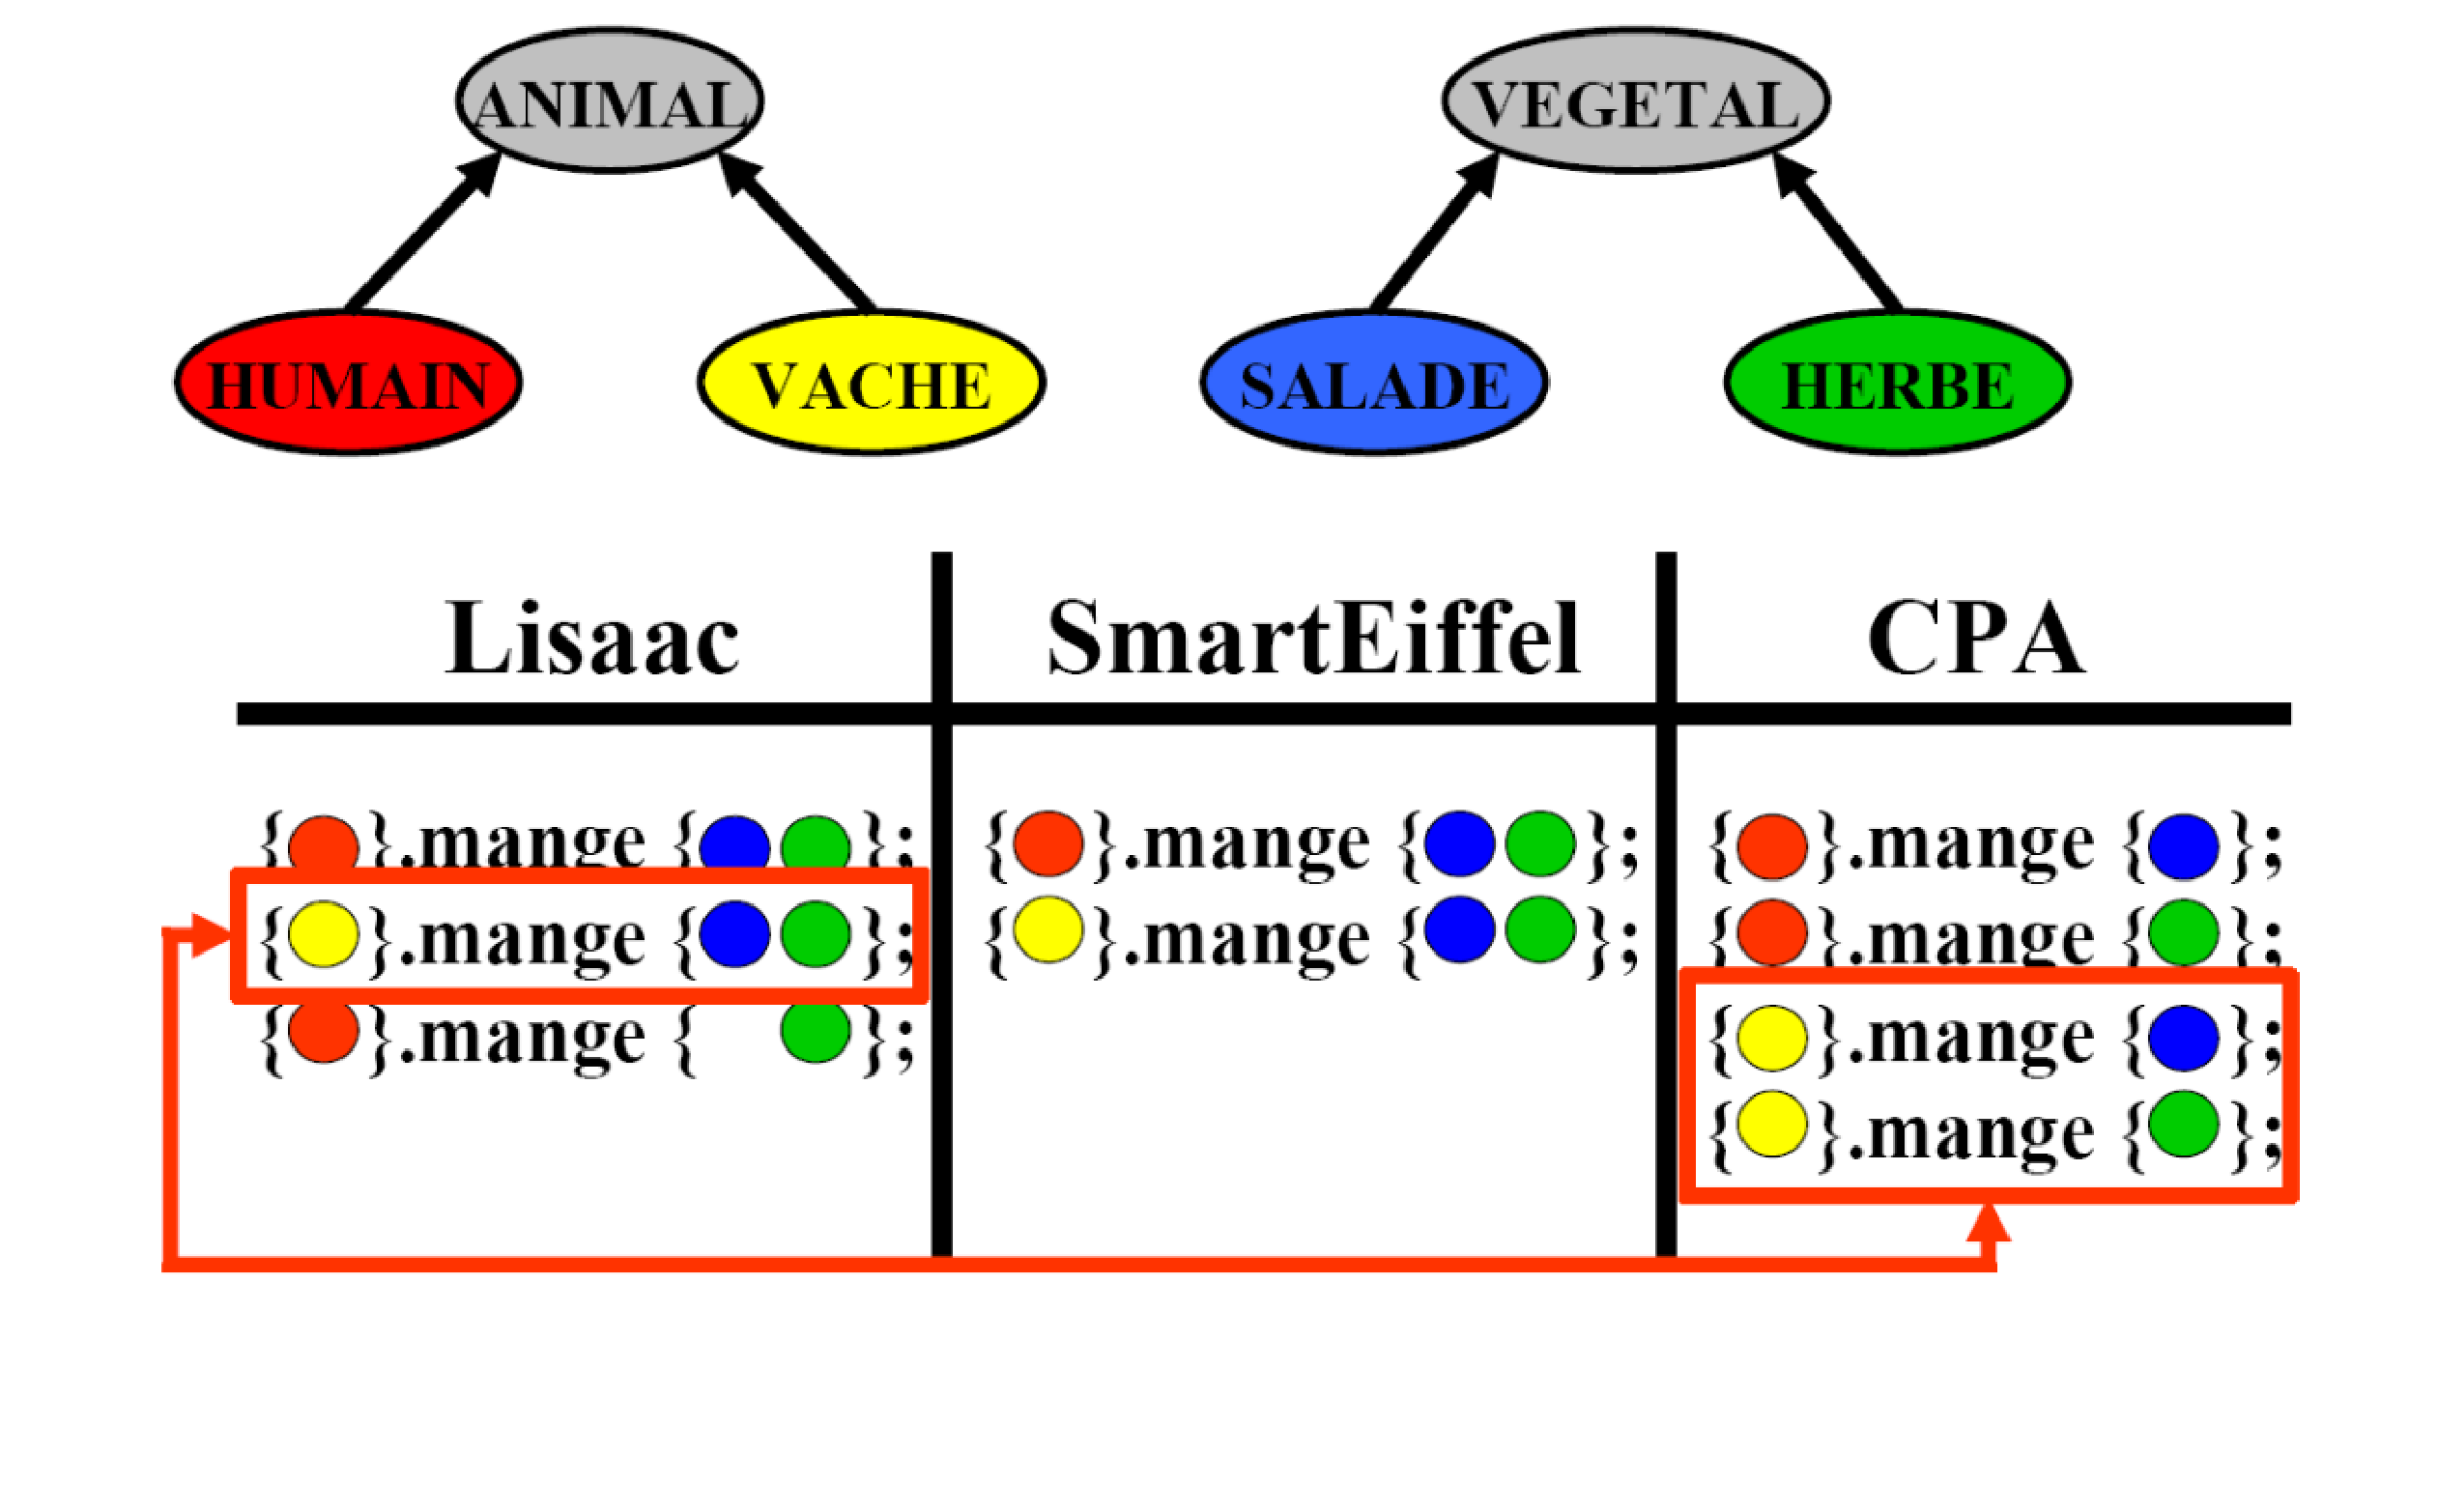
\includegraphics[scale=0.25]{figures/cutomization_7.eps}
\end{frame}
%---------------------------------------------------
\begin{frame}{Customization {\it{}vs} CPA}
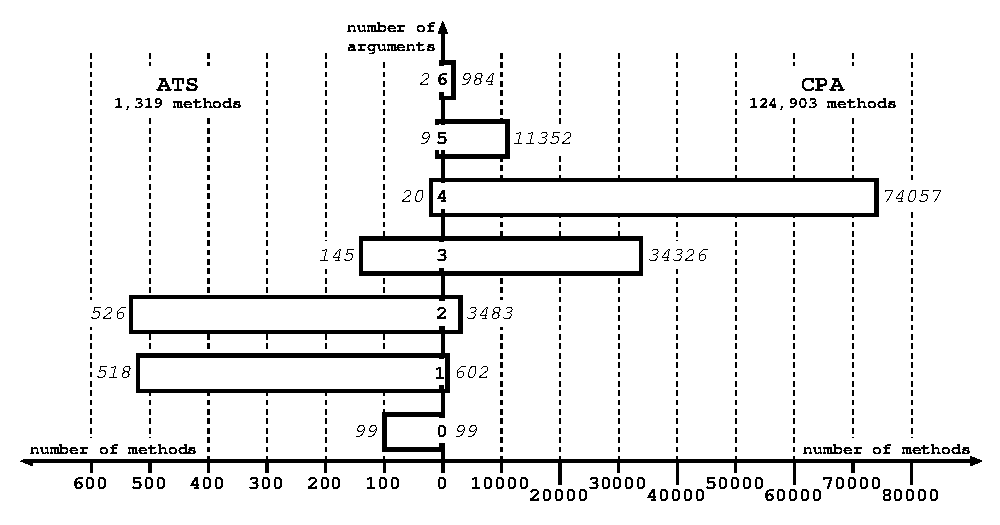
\includegraphics[scale=0.7]{figures/ats_count_vs_cpa_count.eps}
\end{frame}
%---------------------------------------------------
\begin{frame}{Array: Pattern Matching control (1/2)}
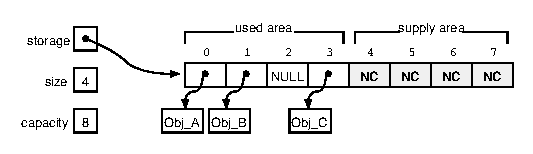
\includegraphics[scale=1.3]{figures/array_count_capacity.eps}
\end{frame}
%---------------------------------------------------
\begin{frame}{Array: Pattern Matching control (2/2)}
\vspace{-0.2cm}
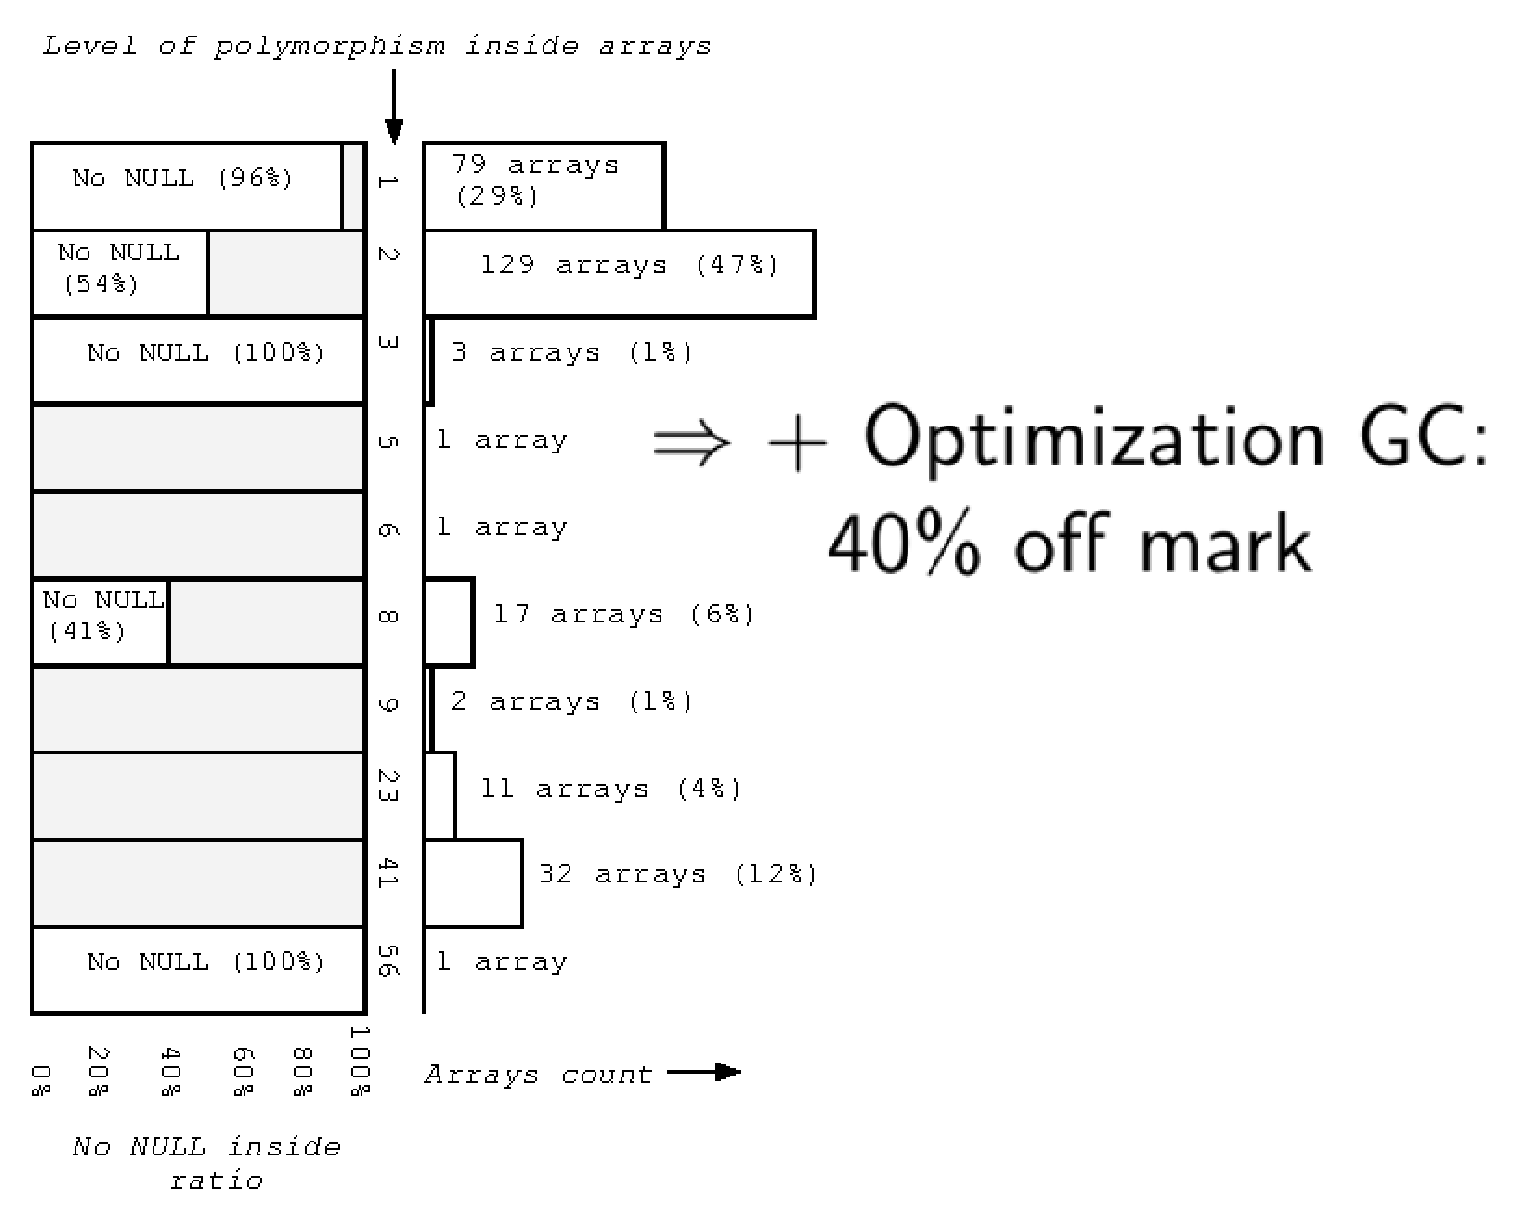
\includegraphics[scale=0.40]{figures/array-type-flow.eps}
\end{frame}
%---------------------------------------------------
\begin{frame}{As fast a C language}
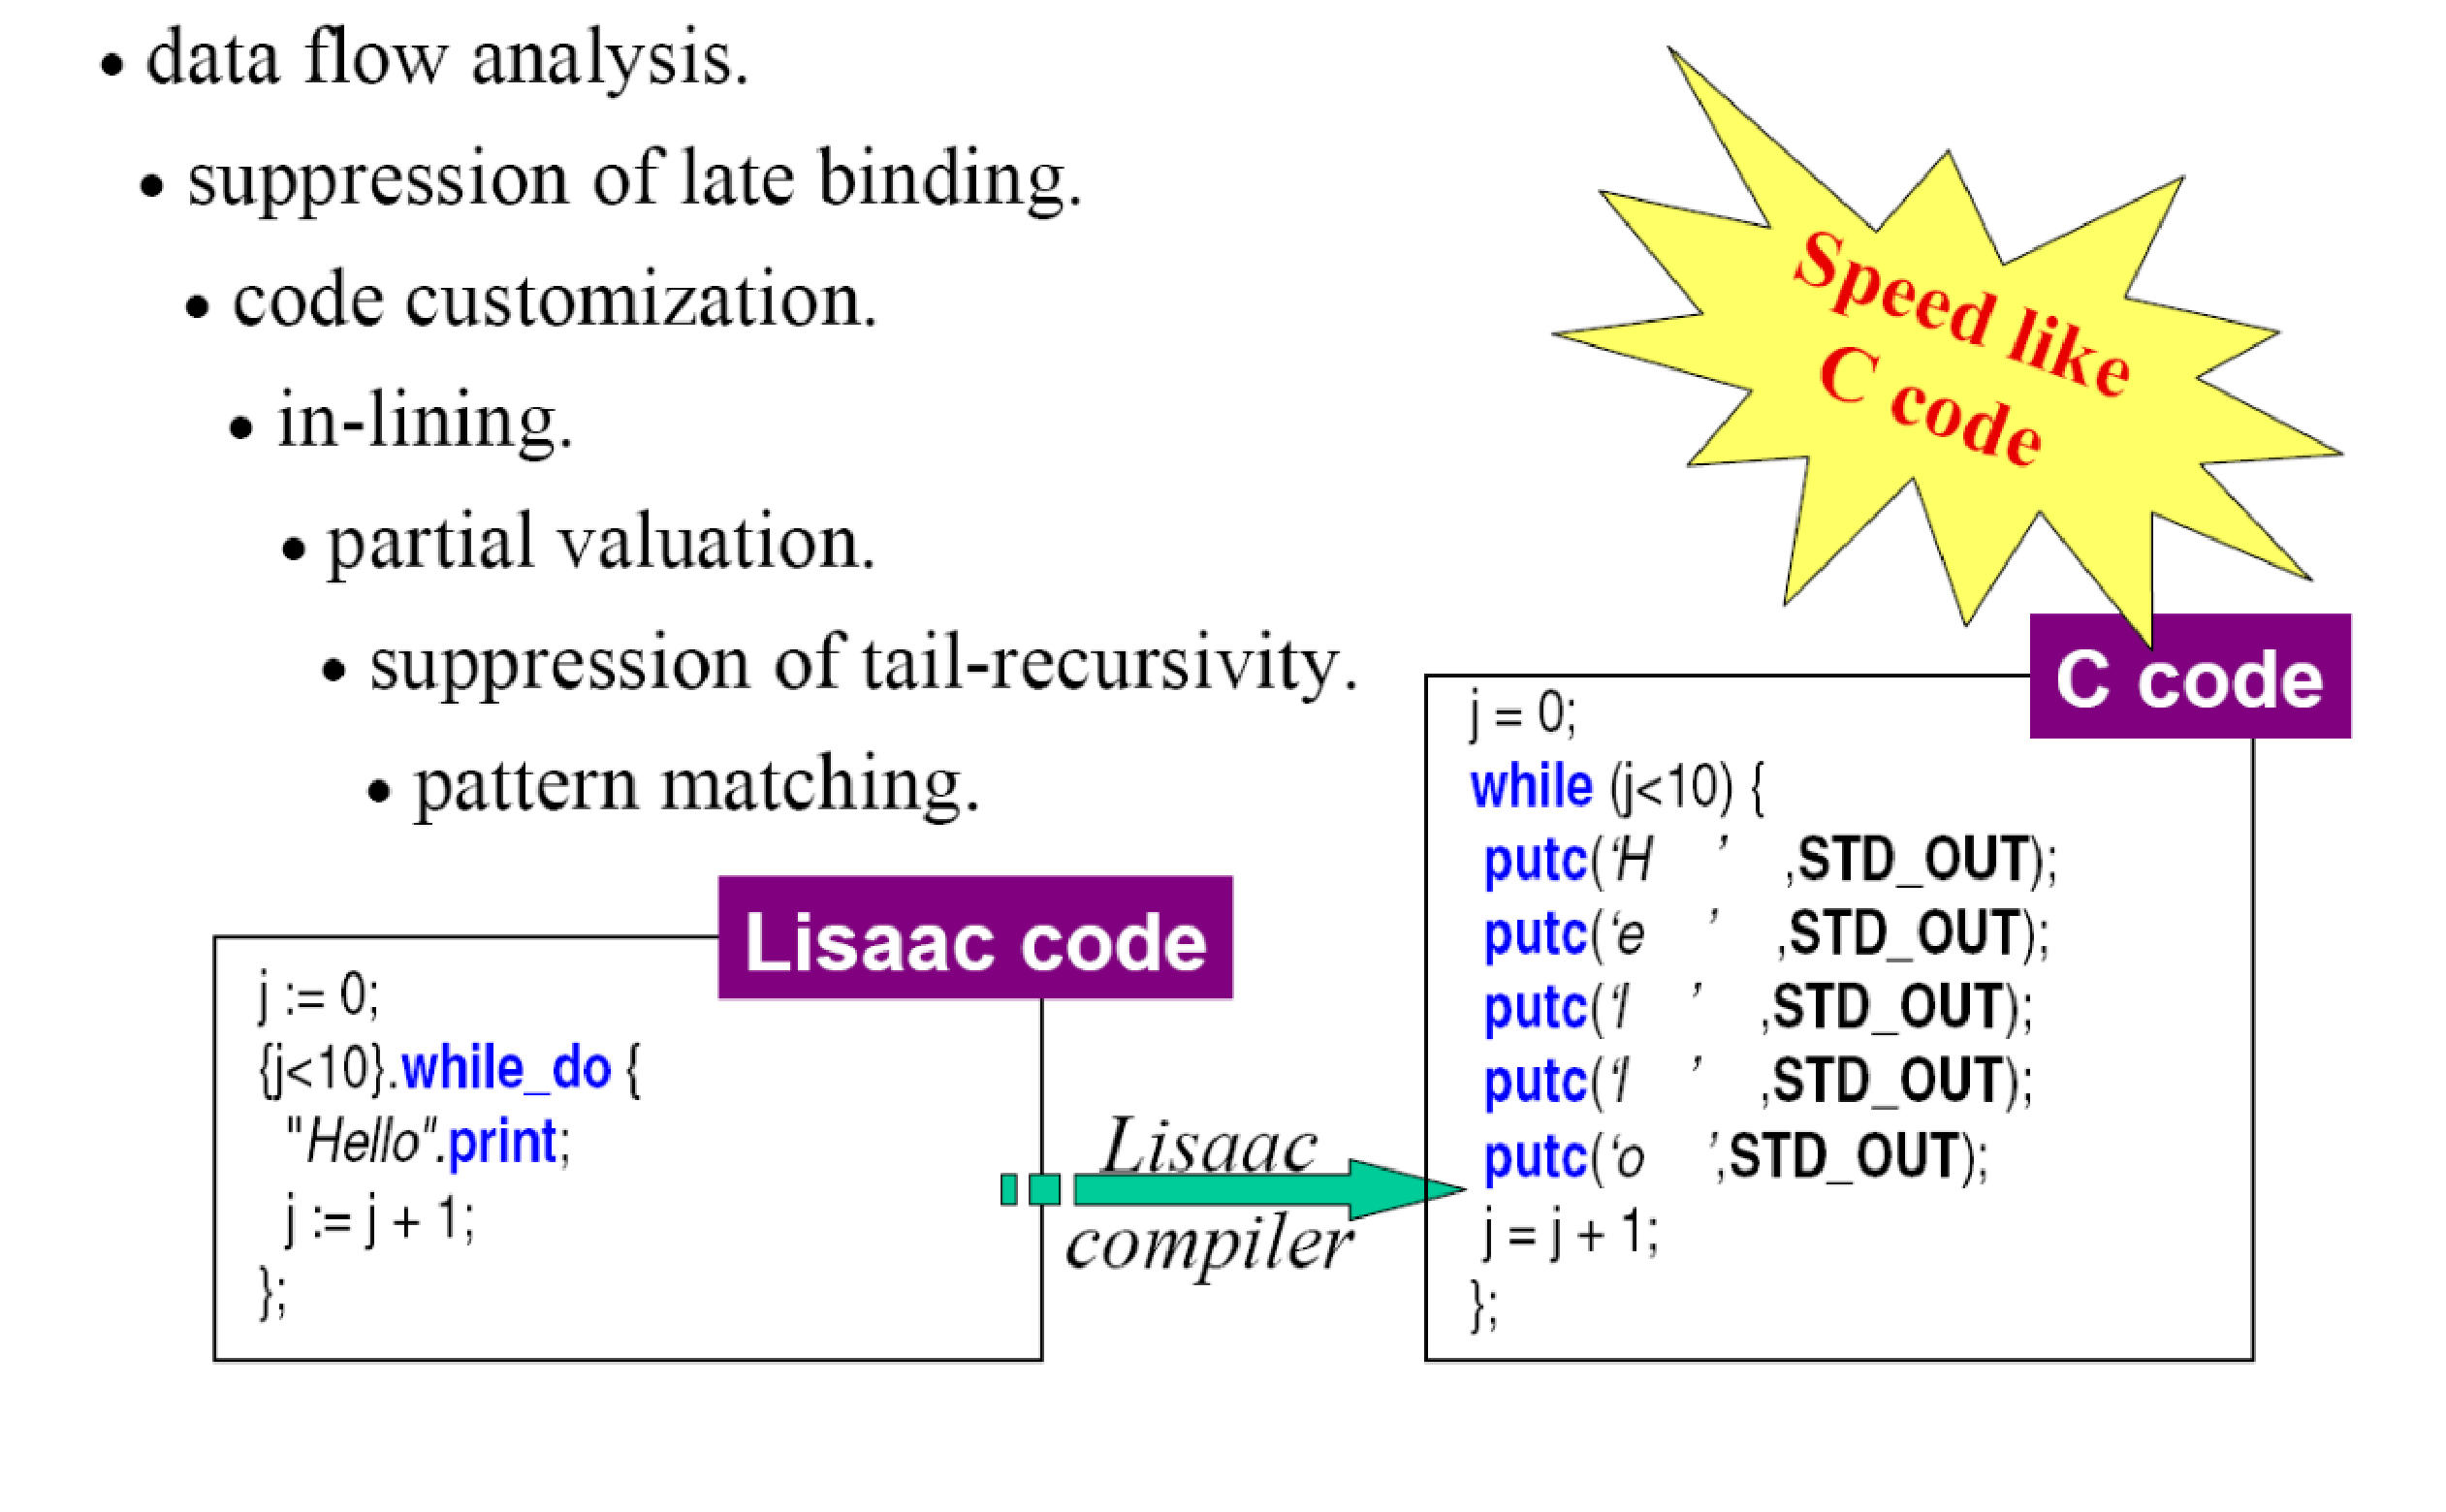
\includegraphics[scale=0.26]{figures/compiler_conclusion.eps}\\
\end{frame}
%---------------------------------------------------

\section{Benchmark}
%===============================
%---------------------------------------------------
\begin{frame}{Tiny test: Quicksort}
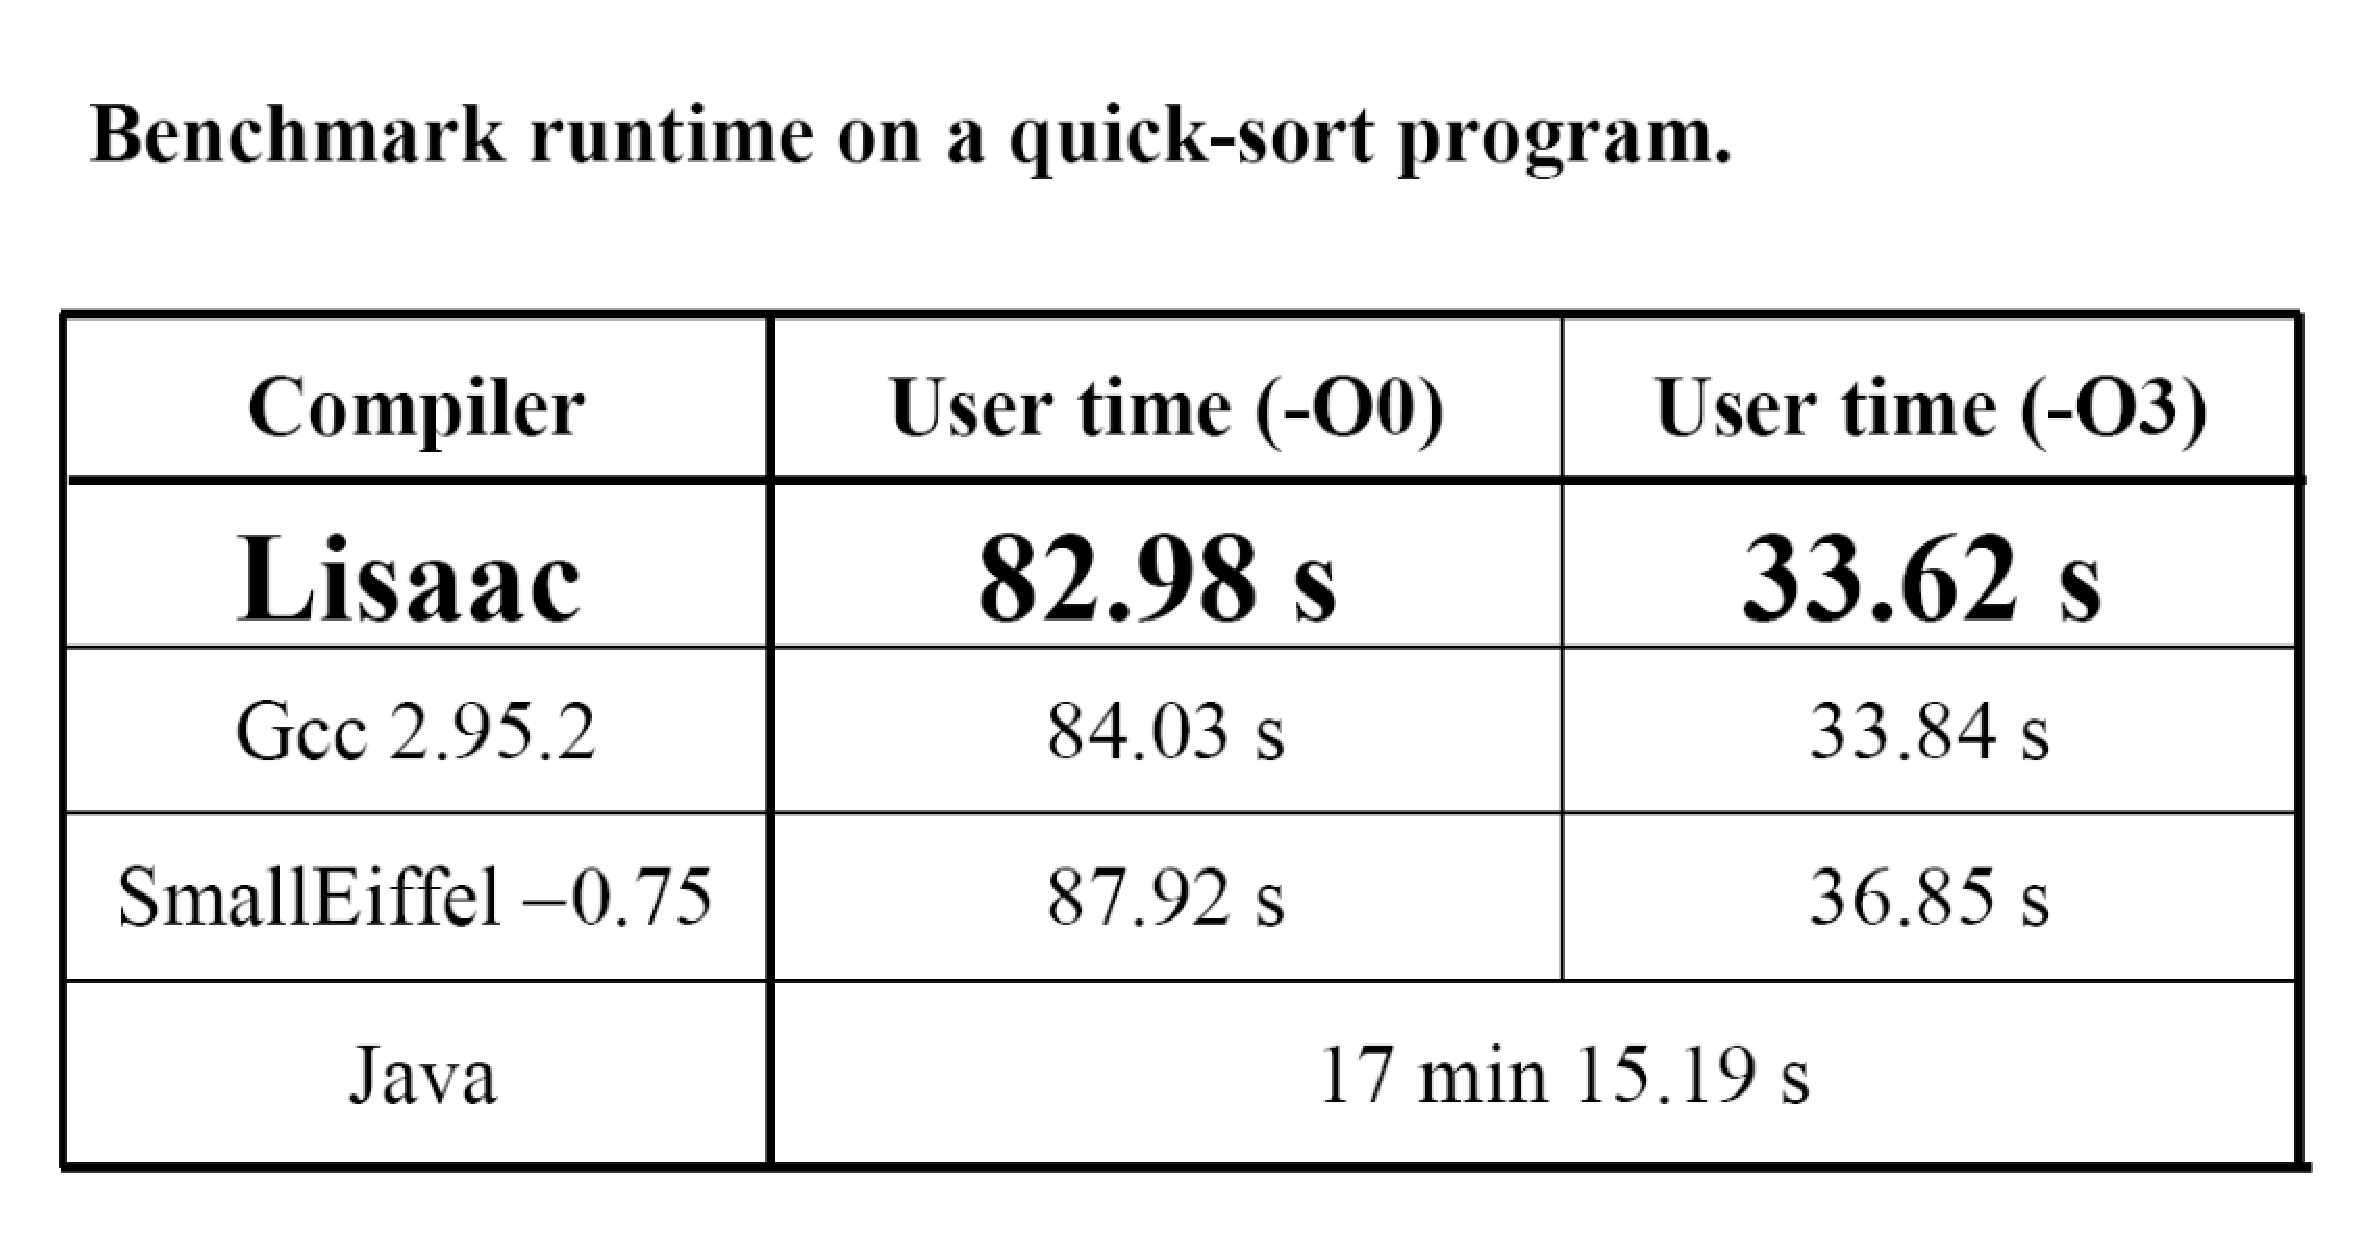
\includegraphics[scale=0.25]{figures/quicksort.eps}
\end{frame}
%---------------------------------------------------
\begin{frame}{Compiler / Bootstrap}
\includegraphics[scale=0.25]{figures/bootstrap.ps}
\end{frame}
%---------------------------------------------------
\begin{frame}{Isaac OS benchmark}
\includegraphics[scale=0.25]{figures/isaac_bench.ps}
\end{frame}
%---------------------------------------------------
\begin{frame}{MPEG2 benchmark}
\includegraphics[scale=0.5]{figures/mpeg2.ps}
\end{frame}
%---------------------------------------------------
\begin{frame}{Shootout benchmark (1/2)}
%\vspace{-2.5cm}
%\hspace{-2.655cm}
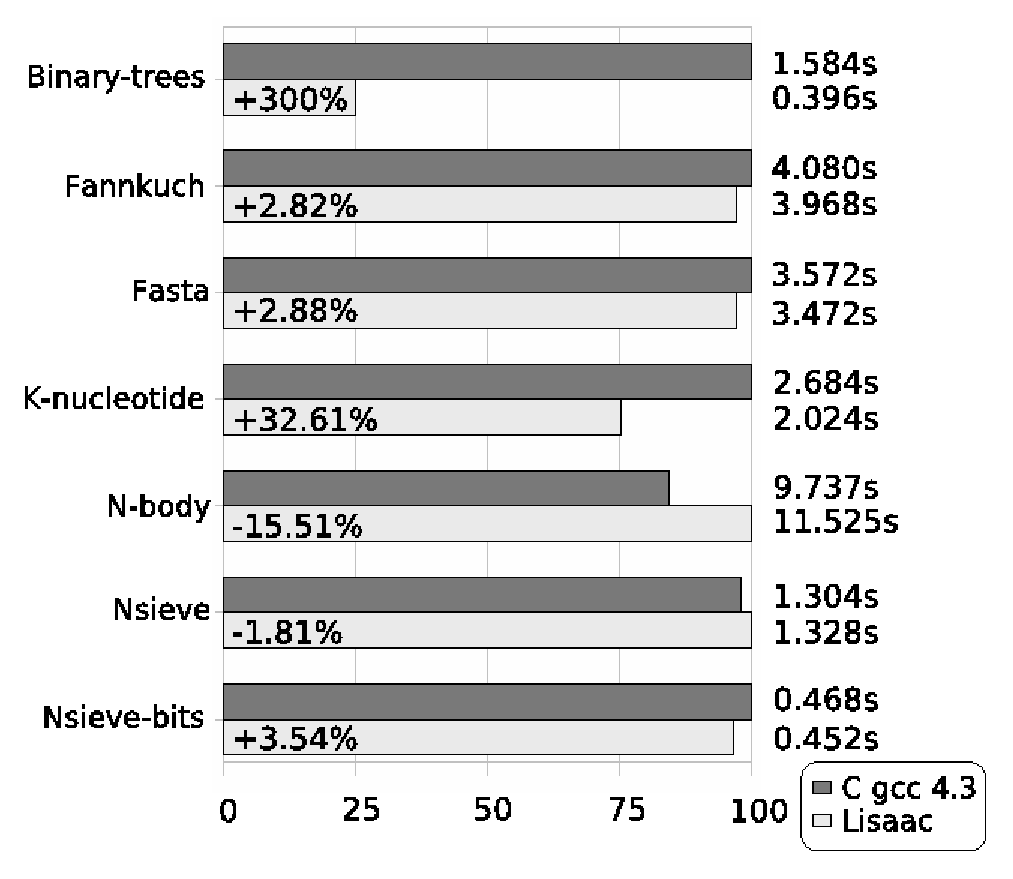
\includegraphics[scale=0.52]{figures/shootout1.eps}
\end{frame}
%---------------------------------------------------
\begin{frame}{Shootout benchmark (2/2)}
%\vspace{-2.5cm}
%\hspace{-2.655cm}
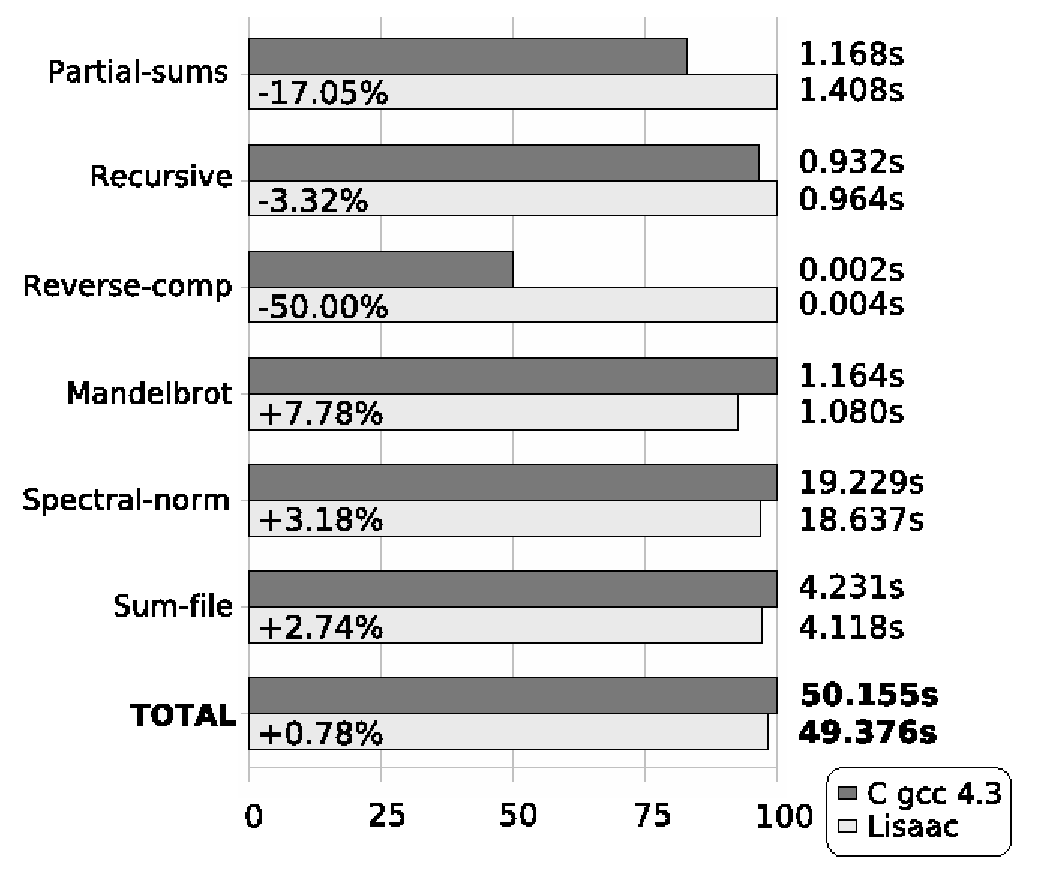
\includegraphics[scale=0.52]{figures/shootout2.eps}
\end{frame}
%---------------------------------------------------
\begin{frame}{Horizontal inheritance}
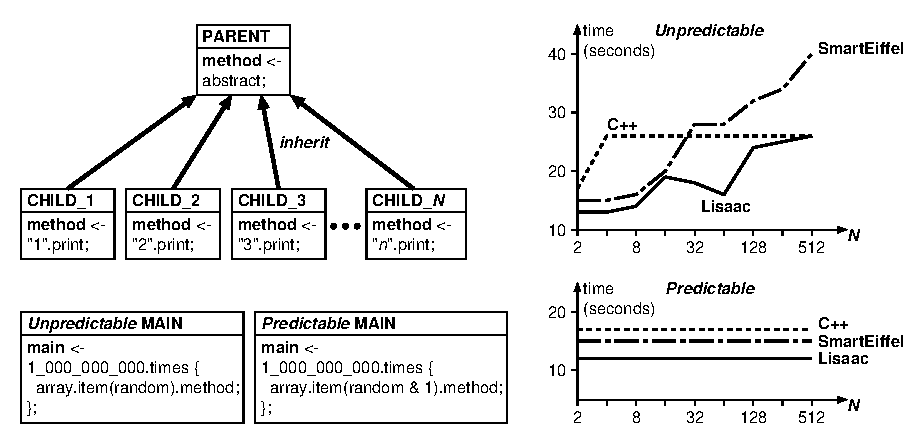
\includegraphics[scale=0.75]{figures/horizontal-bench.eps}
\end{frame}
%---------------------------------------------------
\begin{frame}{Vertical inheritance}
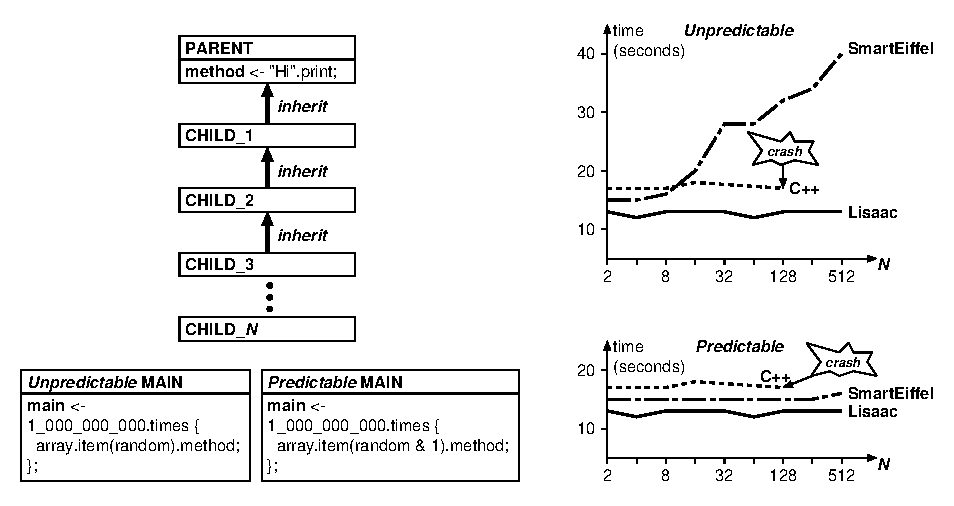
\includegraphics[scale=0.75]{figures/vertical-bench.eps}
\end{frame}
%---------------------------------------------------
\begin{frame}{Auto-cascading}
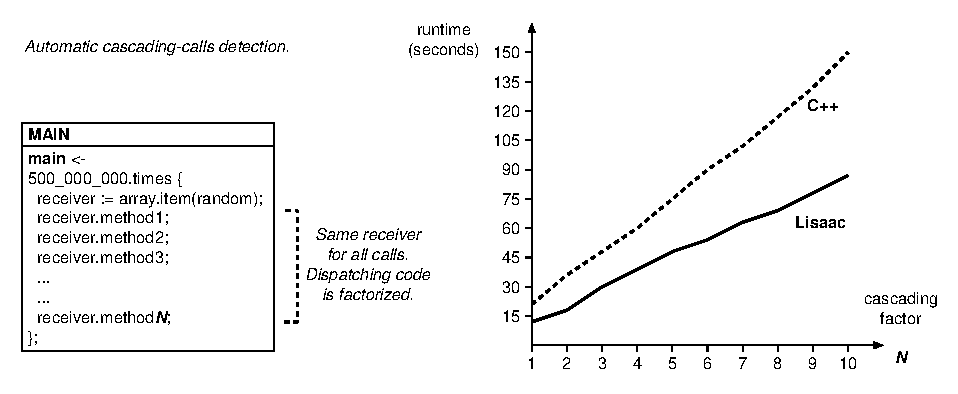
\includegraphics[scale=0.75]{figures/auto-cascading.eps}
\end{frame}
%---------------------------------------------------
\begin{frame}{Call on self {\it{}(this)}}
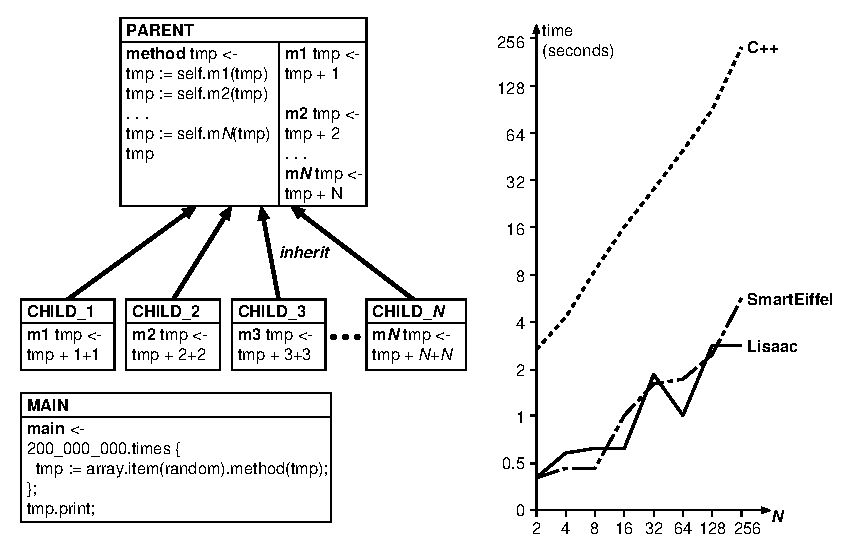
\includegraphics[scale=0.75]{figures/call_on_self_local.eps}
\end{frame}
%---------------------------------------------------
\begin{frame}{Multiple inheritance (1/2)}
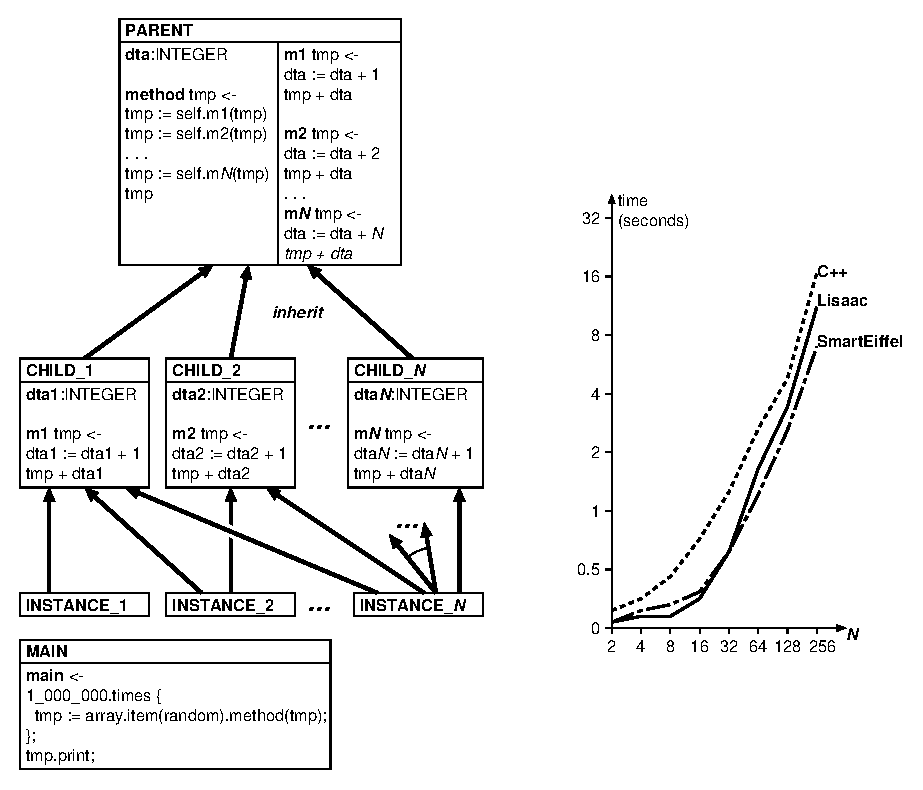
\includegraphics[scale=0.6]{figures/multiple_inheritance.eps}
\end{frame}
%---------------------------------------------------
\begin{frame}{Multiple inheritance (2/2)}
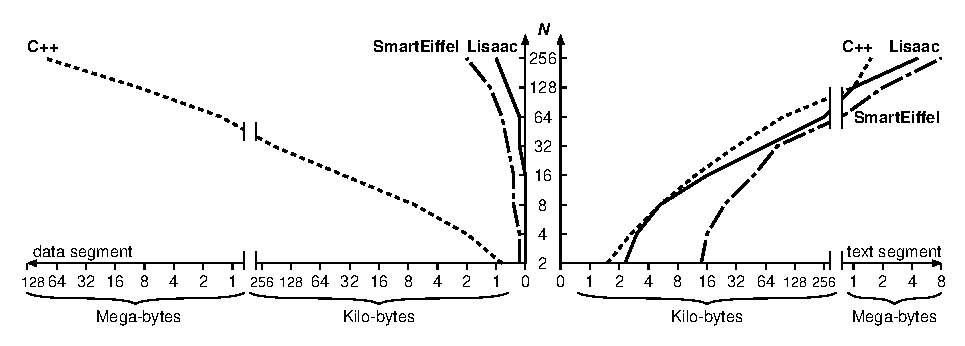
\includegraphics[scale=0.7]{figures/multiple_inheritance2.eps}
\end{frame}

\section{Future}
%===============================
%\begin{frame}{Future\ldots}
%\begin{block}{}
%\begin{itemize}
%\item Site de cr�ation\,: Une mine d'or � exploiter\ldots
%\item Programmation par contrats\,: Information s�mantique encore inexploit�e !
%\end{itemize}
%\end{block}
%$\Rightarrow$ {\it{}Th�se de Matthieu Herrmann}
%\end{frame}

%---------------------------------------------------
\begin{frame}{COP\,: Concurrent Object Prototypes (1/3)}
\begin{center}
\includegraphics{figures/cop-comm.ps}
\end{center}
\end{frame}
%---------------------------------------------------
\begin{frame}{COP\,: Concurrent Object Prototypes (2/3)}
\begin{center}
  \includegraphics[scale=0.65]{figures/cop-clone.ps}
\end{center}
\end{frame}

%---------------------------------------------------
\begin{frame}{COP\,: Concurrent Object Prototypes (3/3)}
\begin{center}
  \includegraphics{figures/cop-assign.ps}
\end{center}
\end{frame}
%---------------------------------------------------
\begin{frame}{COP\,: Concurrent Object Prototypes}
\begin{center}
  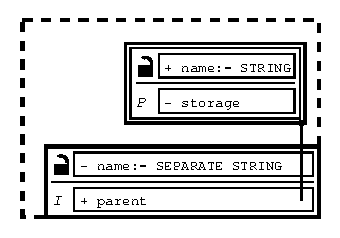
\includegraphics{figures/cop-separate.eps}
\end{center}
\end{frame}

\section{Conclusion}
%===============================
\begin{frame}{Question ?}
\begin{block}{IRC}
\begin{itemize}
\item Server: {\tt{}irc.oftc.net}
\item Channel: {\tt{}\#isaac}
\end{itemize}
\end{block}

\begin{block}{Information \& contacts}
\begin{itemize}
\item {\bf{}Wiki}\,: {\tt{}http://www.lisaac.org/documentation/wiki}
\item {\bf{}Mailing list}\,: {\tt{}lisaac-announce@lists.alioth.debian.org}
\end{itemize}
\end{block}
\begin{center}

\includegraphics[scale=0.5]{figures/isaac_logo.eps} \\
{\tt{}http://www.lisaac.org}
\end{center}
\end{frame}


\end{document}
